% =====================================================================
%  Inscrive Thesis Template  -  main.tex
%  ---------------------------------------------------------------
%  This file only orchestrates: it loads the style, sets metadata and
%  includes content. All styling lives in inscrive-thesis.sty; all
%  prose lives in frontmatter/ and chapters/.
%
%  Build:  pdflatex main  ->  biber main  ->  pdflatex main x2
%          (or just press recompile in Inscrive)
% =====================================================================
\documentclass[12pt,a4paper,oneside]{report}
\usepackage{inscrive-thesis}

% ---- Bibliography database -----------------------------------------
\addbibresource{references.bib}

% ---- Metadata -------------------------------------------------------
\title{GPU-Initiated Communication and Application Scalability}
\subtitle{From microbenchmarks to conjugate gradient application}
\author{Franco Nicolas Merenda}
\studentid{0522501614}
\degree{Master's Degree in Computer Science}
\department{Department of Computer Science}
\university{University of Salerno}
\supervisor{Prof.\ Biagio Cosenza}
\cosupervisor{PhD.\ Lorenzo Carpentieri}
\academicyear{2025--2026}
\keywords{GPU-Initiated Communication, Distributed GPU Computing, MPI, NCCL, oneCCL, NVSHMEM, OSHMPI, UCX, UCC, Conjugate Gradient}

\setcounter{tocdepth}{2}
\setcounter{secnumdepth}{3}

\begin{document}

% ---- Cover ----------------------------------------------------------
% Cover page. Layout is defined by \makecover in inscrive-thesis.sty.
\makecover


% ---- Front matter (roman numerals) ---------------------------------
\pagenumbering{roman}
\frontchapter{Abstract}
As AI model training scales across growing numbers of GPUs, communication becomes a bottleneck. Most communication is host-orchestrated: launches and synchronization can leave devices waiting. GPU invocation moves control into kernels, while only some transports additionally let the GPU post network work directly to the NIC. Neither property is inherently faster; pattern, size, topology, synchronization, and progress determine the result. This thesis characterizes complete communication paths and tests which observations remain valid in a Conjugate Gradient (CG) solver on the Leonardo Booster partition.

We develop \emph{gpu-comm-benchmark}, a CUDA/SYCL suite comparing MPI, NCCL/oneCCL, NVSHMEM, and OSHMPI across point-to-point, halo, collective, and CG-inspired patterns. We also extend oneCCL with grouped NCCL point-to-point, an OSHMPI backend for the benchmarked world-communicator operation set, and a validated NVSHMEM runtime and staging foundation, and extend aCG with OSHMPI and SYCL implementations.

Experiments on 1--32 GPUs expose a decision boundary rather than one winner. MPI minimizes startup cost; persistent, kernel-invoked NVSHMEM leads large steady multi-node halos; NCCL paths lead large allreduce and multi-node all-to-all. MPI/UCC avoids a 17--34$\times$ small-message all-to-all slowdown at 16 and 32 ranks, while its larger multi-node allreduce configurations benefit above a size-dependent crossover around 64\,KiB. In the reconciled synthetic \texttt{cg\_step} archive, OSHMPI has the lowest point estimate in 25 of 30 multi-rank cells, including every multi-node cell, but its archived scalar result remains in host memory; NCCL leads the remaining five and the single-GPU controls.

Comparing \texttt{cg\_step} with aCG gives 7.8--11.1\% mean absolute discrepancy for the matched MPI and NCCL scalar-reduction intervals. The regular synthetic halo misses the application's irregular peers and overlap, and the archived OSHMPI paths also differ in scalar primitive and result placement. NCCL has the lowest representative host-initiated solver times. Device-side NVSHMEM uses CPU-proxy-assisted inter-node networking and improves relative to blocking OSHMPI at larger rank counts but remains behind NCCL. The evidence therefore supports configured performance regimes and selective primitive-level agreement, not an initiation-only speedup; complete application selection requires matching communication structure and completion dependencies.

\printkeywords

\tableofcontents
\listoffigures
\listoftables

% ---- Main matter (arabic numerals) ---------------------------------
\cleardoublepage
\pagenumbering{arabic}
\chapter{Introduction}\label{ch}

\section{Selecting Communication Stacks for Distributed GPU Applications}

Graphics Processing Units (GPUs) provide the parallelism and memory bandwidth used by scientific simulations and large-scale artificial-intelligence training and inference. As these workloads grow beyond one accelerator, they also require more communication: GPUs exchange gradients, activations, parameters, and routed tokens within a node and across cluster interconnects. Pilz et al.'s dataset of 500 AI supercomputers from 2019 to 2025 documents rapid growth in advertised computational capacity, hardware cost, and power demand \cite{pilz_trends_2025}. Those infrastructure trends motivate the scale of the problem; they do not by themselves establish an application communication bottleneck. At application level, performance depends on how data movement and synchronization interact with computation \cite{unat_landscape_2026,choi_end--end_2020}.

Exascale system throughput \cite{top500_june2026} does not remove this coordination problem. Even when a transfer accesses GPU memory directly, the CPU may still issue the operation, wait for a producing kernel, and arrange completion before the next kernel starts. Repeated host orchestration can leave devices idle or prevent useful overlap. Conversely, a host-driven library can remain efficient when its algorithms, batching, and progress mechanisms match the workload. The question is therefore when moving communication control into GPU kernels improves the critical path, rather than whether a system supports direct GPU data movement at all \cite{unat_landscape_2026,agostini_gpudirect_2018}.

This demand has accelerated the development of several programming models and communication libraries. MPI remains the predominant standard for distributed-memory programming and provides a portable interface for point-to-point and collective communication. GPU-aware MPI implementations additionally allow communication operations to access device memory directly, avoiding explicit staging through host memory.

Vendor-optimized collective libraries, such as NVIDIA NCCL and AMD RCCL, provide specialized implementations of operations such as all-reduce, broadcast, reduce-scatter, and all-gather. These libraries are particularly important in distributed deep-learning workloads, where collective operations frequently dominate communication time \cite{weingram_xccl_2023}. Their performance depends on several internal decisions, including the selected communication algorithm, transport protocol, number of communication channels, and underlying system topology \cite{hu_demystifying_2025}.

A different approach is provided by one-sided Partitioned Global Address Space models such as OpenSHMEM. GPU-oriented implementations, including NVSHMEM and ROC\_SHMEM, extend this model by allowing communication operations to be initiated directly by GPU threads or thread blocks. Device-initiated communication can reduce CPU involvement and enable fine-grained communication from inside a kernel, potentially improving overlap and reducing synchronization overhead \cite{agostini_gpudirect_2018,ma_demystifying_2026}. Portable implementations such as OSHMPI instead provide OpenSHMEM semantics over MPI. These alternatives make different trade-offs: symmetric-memory requirements, synchronization semantics, message granularity, host involvement, and implementation maturity can all determine whether one-sided communication is beneficial.

Recent work has demonstrated that default collective algorithms and runtime configurations can be significantly slower than configurations selected for a particular topology and workload \cite{pasqualoni_pico_2026,li_tuccl_2025}. The communication backend should therefore be treated as a workload-dependent design choice rather than as an interchangeable implementation detail.

The rapid growth of this ecosystem creates a practical selection problem. MPI, NCCL, oneCCL, NVSHMEM, and OSHMPI expose different interfaces and may use different algorithms, progress engines, memory requirements, and transports. Their names alone do not tell an application developer which stack will perform best. The answer depends on the application's communication signature: the operations it issues, their message sizes, peer sets, synchronization points, rank placement, and opportunities for computation--communication overlap.

Vendor-specific ecosystems generally provide highly optimized implementations, but they couple applications to a particular hardware and software stack. SYCL and oneCCL provide source-level abstractions that reduce this coupling. Source portability, runtime backend interchangeability, and performance portability are nevertheless distinct properties: a common interface may add orchestration, staging, or synchronization costs, and measurements on NVIDIA A100 GPUs cannot by themselves establish cross-vendor performance portability \cite{hammond_comparative_2019,shen_sycl_2026}. This thesis therefore treats CUDA and SYCL variants as concrete implementation stacks and supporting controls, rather than making cross-vendor portability a separate experimental claim.

\subsection{Research Gap and Approach}

Prior work already connects communication mechanisms to applications. Agostini et al. examine GPUDirect Async through microbenchmarks, modeling, and application cases; PICO assesses benchmark-informed choices through simulated training-trace replay; TuCCL reports end-to-end training improvements; and Trotter et al. compare host- and device-initiated CG solvers \cite{agostini_gpudirect_2018,pasqualoni_pico_2026,li_tuccl_2025,trotter_cpu-_2025}. The gap addressed here is the specific combination of a common CUDA/SYCL comparison across MPI, collective-library, and SHMEM paths with measured validation in an extended sparse solver. Supporting that comparison also requires functionality absent from the selected software baselines: oneCCL lacks the added OSHMPI and NVSHMEM paths and complete grouped NCCL dispatch, while the published aCG suite provides CUDA/HIP implementations without the OSHMPI communicator or SYCL port developed here.

This thesis addresses those gaps through a pattern-oriented workflow. It first compares configured host- and GPU-initiated paths to locate favorable regimes. It extends oneCCL with grouped NCCL support and an OSHMPI backend, and establishes a separately validated NVSHMEM runtime foundation. Finally, OSHMPI and SYCL extensions to aCG test the benchmark guidance in a complete sparse solver. The central hypothesis is conditional: persistent device work can amortize host-control costs, but memory placement, completion semantics, proxy progress, and application dependencies determine whether that opportunity becomes a performance benefit. Comparisons of complete stacks identify useful candidates; they do not isolate initiation as the only changing variable.

This is why the benchmark suite developed in this work is organized around communication patterns rather than around library interfaces. It covers reductions, neighbor exchanges, and all-to-all redistribution because they expose different requirements: reductions combine values globally, neighbor exchanges communicate with a small application-defined set of peers, and all-to-all redistributes distinct data among all ranks. Data-parallel and sharded training motivate the reduction family, Mixture-of-Experts expert routing motivates all-to-all and variable-count redistribution, and iterative sparse solvers motivate latency-sensitive reductions and halo exchanges. A pattern-oriented characterization can therefore inform several workload families without implying that every workload contains every pattern.

\section{Scope and Main Findings}

This thesis applies that workflow on the Leonardo Booster partition. It first measures point-to-point, halo, reduction, and all-to-all patterns across CUDA-aware and SYCL-aware MPI, NCCL, oneCCL, NVSHMEM, and OSHMPI stacks on 1 to 32 NVIDIA A100 GPUs. Most benchmark paths are host-initiated, while the NVSHMEM ping-pong and halo implementations issue communication from persistent cooperative GPU kernels. A composite \texttt{cg\_step} benchmark then combines a host-driven halo exchange with the small reductions characteristic of one Conjugate Gradient iteration. Finally, the study evaluates host-initiated and monolithic device-initiated aCG solvers on two large sparse matrices. Conjugate Gradient combines sparse matrix--vector multiplication, vector operations, halo exchanges, and global reductions; its low computational intensity and repeated synchronization make scalability sensitive to communication overhead \cite{trotter_cpu-_2025}. All-to-all remains a standalone pattern motivated by redistribution-heavy workloads such as Mixture-of-Experts and is not validated by aCG.

The main campaign produces a pattern-specific ranking. HPC-X MPI has the lowest point-to-point and isolated-halo startup cost; device-initiated NVSHMEM leads large steady-state halos; NCCL-based paths lead large allreduce and multi-node all-to-all. MPI/UCC prevents a 17--34$\times$ small-message all-to-all slowdown at 16 and 32 ranks, while its multi-node allreduce effect changes from a penalty below 64\,KiB to a benefit at and above that size. Direct OSHMPI with host-staged scalar reductions wins every multi-rank synthetic \texttt{cg\_step}; NCCL leads the communication-free controls. Chapter~\ref{ch:m-results} explains the completion, staging, and phase-timing qualifications behind these findings.

The predictive value of these benchmarks is tested with aCG. This work adds an OSHMPI communicator whose halo exchange uses OpenSHMEM puts while its scalar CG reductions retain CUDA-aware \texttt{MPI\_Allreduce}. The direct OSHMPI \texttt{cg\_step} instead uses OpenSHMEM reductions, so those reduction measurements have no matched aCG counterpart. For the matched paths, \texttt{cg\_step} predicts aCG's eight-byte reduction cost within 6.5--9.7\% for MPI and NCCL and within 14--21\% for NVSHMEM across a 16-fold range in process count. In contrast, the regular two-neighbor eager halo does not predict aCG's irregular many-neighbor rendezvous exchange, whose communication is largely hidden by sparse matrix--vector multiplication. NCCL remains the fastest stable host-initiated backend in aCG, while the MPI halo exhibits fast and slow execution regimes that also affect the subsequent allreduce.

A separate monolithic NVSHMEM aCG variant examines GPU-initiated execution and scales better than the blocking OSHMPI path at larger process counts. It also changes solver organization and is therefore not a strict backend substitution. Moreover, Leonardo does not enable IBGDA, so its inter-node RMA uses the \texttt{ibrc} CPU proxy and does not measure GPU-posted inter-node communication. The combined evidence locates the benefit more narrowly than a library ranking: GPU initiation helps persistent neighbor work and can improve solver scaling when it removes repeated host synchronization, but it does not overcome MPI's startup advantage and remains sensitive to proxy progress. Microbenchmarks predict application behavior only when communication primitives, peer structures, completion boundaries, and overlap opportunities are comparable. The rankings are specific to Leonardo; the decision method is reusable on other systems.

A later exploratory \texttt{nccl-tests} comparison examines NCCL~2.18.5 and 2.31.2 with ordinary and symmetrically registered buffers on four GPUs within one node. Its summary indicates promising small-allreduce improvements, with regressions at other sizes and little small-message all-to-all benefit. Section~\ref{sec:nccl-preliminary-results} reports this as a separate preliminary study: the available summary does not establish the selected kernel or application-visible initiation mode, and these measurements do not revise the main campaign's rankings.

\section{Research Questions}

The investigation follows the same progression as the contributions. It first establishes a common comparison across communication models, then asks what is required to expose missing paths through oneCCL, and finally tests the benchmark guidance after extending a complete solver. This ordering makes the novelty relative to the baseline software explicit:

\begin{researchquestion}[RQ1 -- Conditions for beneficial GPU initiation]
Under which communication patterns, message sizes, topologies, and completion regimes do the evaluated GPU-initiated paths become beneficial relative to host-initiated stacks, and what evidence supports launch, synchronization, or proxy-progress costs as explanations for the observed boundaries?
\end{researchquestion}

\begin{researchquestion}[RQ2 -- Extending oneCCL beyond its baseline backends]
Compared with the baseline oneCCL backend set, what functionality and semantic adaptations are required for grouped NCCL point-to-point, OSHMPI/OpenSHMEM execution, and an NVSHMEM backend foundation, and what asynchrony, staging, portability, and readiness trade-offs result?
\end{researchquestion}

\begin{researchquestion}[RQ3 -- Transfer to extended CG solvers]
After extending aCG with OSHMPI and SYCL implementations, to what extent do the benchmark's host-versus-GPU-initiation findings transfer to complete CG solvers, and how do irregular peers, synchronization, computation--communication overlap, memory placement, and solver organization explain agreement or failure?
\end{researchquestion}

\section{Major contributions}

\begin{keypoint}[Central proposition]
GPU initiation is a mechanism, not a performance guarantee. Persistent device work can amortize launch costs and reduce repeated host synchronization, while application overlap can hide communication. These opportunities pay off only when the resulting cost is lower than the competing path. Pattern-oriented microbenchmarks locate candidate regimes; a complete application checks whether peers, completion semantics, and dependencies preserve them.
\end{keypoint}

To answer these questions, this thesis makes five main contributions. The second and third extend oneCCL beyond the baseline backend behavior, while the fourth and fifth extend aCG beyond the published CUDA/HIP suite.

\begin{enumerate}

\item \textbf{A unified benchmark across vendor-specific and portable APIs.}
A set of representative communication patterns characterizes latency, bandwidth, synchronization overhead, message-size sensitivity, and topology-dependent behavior across seven runtime stacks. Unlike separate per-library tests, the harness applies common process-to-GPU mapping, warm-up, measurement, validation, and result-reduction policies to CUDA- and SYCL-based MPI, NCCL/oneCCL, NVSHMEM, and OSHMPI paths. Its NVSHMEM ping-pong and halo kernels provide the GPU-initiated cases, while host-initiated stacks establish the comparison surface. Global reductions and neighbor exchanges correspond directly to aCG phases and support RQ3. All-to-all and alltoallv remain standalone redistribution patterns motivated by deep-learning workloads. The design spans vendor-specific and portable interfaces, while the reported validation remains specific to NVIDIA A100 GPUs. The suite is available at \url{https://github.com/y3rbiadit0/gpu-comm-benchmark}.

\item \textbf{Grouped point-to-point support for the oneCCL NCCL backend.}
oneCCL exposes \texttt{ccl::group\_start} and \texttt{ccl::group\_end} so that a sequence of operations can be submitted as one batch. For the NCCL backend, grouping is required to submit mutually dependent point-to-point operations together and is also a performance mechanism: NCCL can execute the batch in one launch and assign grouped transfers to separate channels where possible \cite{hu_demystifying_2025}. Before this work the group lifecycle was implemented only for the native path. This contribution adds backend-aware dispatch to \texttt{ncclGroupStart} and \texttt{ncclGroupEnd}, nested-group handling, events that track the deferred NCCL work, explicit failure propagation, and group-aware send/receive fallbacks for all-to-all. The semantics are documented and covered by dedicated grouped point-to-point tests. The implementation is available at \url{https://github.com/y3rbiadit0/oneCCL/tree/fix/nccl_group_support}.

\item \textbf{SHMEM-family backend extensions for oneCCL.}
The complete OSHMPI path, selected with \texttt{CCL\_BACKEND=oshmpi}, adds backend discovery, communicator and rank validation, datatype and reduction mapping, collective implementations, symmetric staging for ordinary host or SYCL USM buffers, and put-based point-to-point operations with explicit completion. It exposes the practical cost of mapping oneCCL's asynchronous event interface onto blocking, host-driven OpenSHMEM operations and is measured in the benchmark. A separate \texttt{CCL\_BACKEND=nvshmem} prototype establishes optional build integration, CUDA-backed SYCL communicator selection, KVS-distributed UID bootstrap, ownership-safe lifecycle handling, and a fixed symmetric staging arena. Its runtime and staging foundation passed one- and two-node validation, but its oneCCL collective entry points remain explicitly unsupported and it contributes no performance data. The implementations are available at \url{https://github.com/y3rbiadit0/oneCCL/tree/feat/oshmpi} and \url{https://github.com/y3rbiadit0/oneCCL/tree/feat/nvshmem_collectives}.

\item \textbf{An OSHMPI communicator and application validation in aCG.}
The aCG solver is extended with an OSHMPI communicator to test whether benchmark-level one-sided halo results transfer to a complete sparse solver. The communicator uses OpenSHMEM for halo exchange while retaining CUDA-aware \texttt{MPI\_Allreduce} for scalar reductions, so the application comparison does not treat the direct OSHMPI \texttt{cg\_step} benchmark's OpenSHMEM reductions as a matched primitive. The solver is evaluated against its MPI, NCCL, host-NVSHMEM, and device-NVSHMEM variants. The complete campaign connects the benchmark patterns to sparse matrix--vector multiplication, overlap, synchronization, and convergence on two large SuiteSparse matrices. The communicator is available at \url{https://github.com/y3rbiadit0/aCG-oshmpi/tree/oshmpi}.

\item \textbf{A SYCL implementation of aCG.}
The CUDA-oriented application is additionally implemented through SYCL, with distributed execution through MPI and selectable MPI or oneCCL scalar reductions. This port provides a complete portable-compute control for determining whether kernel and orchestration costs can dominate a communication comparison. Its evaluation is kept separate from the CUDA communicator campaign and is used as supporting evidence rather than as a claim of cross-vendor performance portability. The implementation is available at \url{https://github.com/y3rbiadit0/acg-sycl}.

\end{enumerate}

\section{Thesis Organization}

Chapter~\ref{ch:m-problem} introduces the hardware, communication patterns, programming models, libraries, transports, and performance concepts required to interpret the measurements. Chapter~\ref{ch:m-methodology} maps research questions to artifacts and evidence, then describes the benchmark, aCG campaign, tuning, and preliminary NCCL protocol. Chapter~\ref{ch:m-results} reports microbenchmark, composite-step, and complete-solver evidence, followed by the separate exploratory NCCL comparison. Chapter~\ref{ch:m-related} positions the work relative to communication characterization, GPU initiation, and application-level studies. Chapter~\ref{ch:m-discussion} answers the research questions and states the threats to validity. The final chapter summarizes the conclusions and identifies the questions that require further experiments.


\chapter{Background}\label{ch:m-problem}

This chapter builds the decision model used throughout the thesis. An application first produces a \emph{communication signature}: a pattern of operations with particular message sizes, rank counts, placements, dependencies, and synchronization requirements. A programming interface expresses that signature; a library implementation selects algorithms and protocols; a transport maps them to physical links; and the hardware topology determines the available routes and their costs. Performance is therefore a property of the complete chain rather than of a library name in isolation.

The chapter follows these dependencies from hardware upward. Interconnects determine what data movement is physically possible and at what cost. Programming models determine how computation is expressed and which vendor stacks an application is tied to. Communication operations define the transformations requested by an application without prescribing their schedules. Libraries then decide how those requests become traffic on the interconnect, while compilers and toolchains determine which combinations can actually be built. Throughout this thesis, \emph{model} denotes semantics such as two-sided message passing or one-sided PGAS; \emph{implementation} denotes a concrete library such as HPC-X MPI, NCCL, or NVSHMEM; \emph{oneCCL backend} denotes the adapter selected beneath oneCCL; and \emph{transport} denotes the provider that ultimately moves the data, such as shared memory, TCP, CUDA IPC, UCX, or InfiniBand verbs. The chapter closes with the performance concepts used to interpret the measurements and with a description of the evaluation platform.

\section{GPU-Centric Communication and Interconnects}\label{sec:interconnects}

A multi-GPU application communicates across two domains with different physical substrates, different cost structures, and different software mechanisms: \emph{intra-node}, between GPUs sharing a chassis, and \emph{inter-node}, between GPUs in different chassis connected by a network. This section treats them in turn. Within each, the discussion separates the \emph{interconnect} -- what the hardware physically provides -- from the \emph{communication types} it supports, meaning the distinct routes a transfer can take and the distinct division of labor between GPU, CPU, and network adapter that each route implies. The distinction matters because a single interconnect supports several types, the type actually used is chosen by the software stack rather than by the application, and the difference between two types on identical hardware can exceed an order of magnitude.

\subsection{Invocation, Progress, and Memory Are Separate Axes}\label{sec:initiation-axes}

\emph{GPU-aware} describes an interface's ability to accept device buffers; \emph{GPU-initiated} describes where an operation is invoked. Neither term specifies who posts a network request or whether communication overlaps computation. Table~\ref{tab:m-initiation-axes} keeps these distinctions explicit. In particular, a CPU-launched communication kernel is not evidence that the application itself calls a communication API from GPU code, and a device-side call may still depend on a CPU progress thread \cite{unat_landscape_2026,hamidouche_kernel-initiated_2026}.

\begin{table}[htbp]
\centering
\caption{Independent dimensions needed to interpret a GPU communication path.}
\label{tab:m-initiation-axes}
\scriptsize
\begin{tabularx}{\textwidth}{lYY}
\toprule
Dimension & Meaning & Example or limitation\\
\midrule
Host invocation & CPU issues the operation & GPU-aware MPI accepts device memory without becoming device-initiated\\
Host-on-stream & CPU enqueues ordered work & NCCL host collectives and NVSHMEM on-stream calls can be asynchronous\\
Device invocation & Kernel calls communication primitives & NVSHMEM persistent neighbor kernels; NCCL user device API\\
Proxy progress & CPU posts requests generated by GPU code & Evaluated inter-node NVSHMEM \texttt{ibrc}; a device call still uses CPU resources\\
Direct NIC posting & GPU constructs/posts network work & IBGDA or NCCL GDAKI, subject to version-specific prerequisites\\
Memory/access & Allocation, registration, and peer reachability & Peer mappings enable remote loads/stores; registration alone does not establish invocation mode\\
\bottomrule
\end{tabularx}
\end{table}

These dimensions must be identified together when interpreting a measurement. A GPU kernel may access peer memory directly within a node yet rely on a CPU proxy for a remote node, while a host-called operation may use the same registered memory as a device-called one. The NCCL discussion in Section~\ref{sec:xccl} illustrates these combinations through its device API and symmetric-memory support. The following subsections establish the intra-node and inter-node mechanisms on which such interfaces depend.

\subsection{Intra-Node Communication}\label{sec:intra-node}

\subsubsection{The Interconnect}

Within a node, GPUs are connected either through PCI Express or through a dedicated high-bandwidth fabric. PCIe is general-purpose and shared with storage and network devices; even at version 6.0 its bidirectional bandwidth of roughly 256\,GB/s remains much lower than local HBM bandwidth, which already exceeds 3\,TB/s on an H100-class device \cite{song_survey_2025}. Communication-intensive multi-GPU workloads can therefore encounter a large gap between local memory access and peer data movement. Vendor fabrics were introduced to narrow it. NVLink provides direct point-to-point links between GPUs and has scaled aggressively across generations, from 160\,GB/s of bidirectional bandwidth in NVLink~1.0 to 1800\,GB/s in NVLink~5.0; NVSwitch extends the fabric into a switched all-to-all topology, connecting eight GPUs at 4.8\,TB/s aggregate in the NVSwitch~2.0 generation that accompanies the A100 \cite{song_survey_2025}. AMD's equivalent is Infinity Fabric with xGMI links, and the field is now broadening: UALink, OISA, SUE, and further proprietary \mbox{X-Link} designs target the same ``scale-up'' domain, and their protocol-level differences are surveyed in \cite{song_survey_2025}.

An important distinction is that per-device figures aggregate all of a GPU's links; they are not automatically the bandwidth available between one pair of GPUs. The A100 devices used in this work expose NVLink~3.0 as 12 links of 25\,GB/s per direction, giving 600\,GB/s of bidirectional endpoint bandwidth in total. Pair bandwidth depends on how those links are distributed and routed. NVSwitch provides switched connectivity, but a transfer remains bounded by endpoint, switch, and concurrent-traffic limits. The Leonardo Booster node described in Section~\ref{sec:leonardo} instead connects four GPUs directly, with four links per peer, giving a 200\,GB/s bidirectional theoretical ceiling for one pair -- one third of the per-device aggregate. The distinction matters whenever an aggregate specification is used as the reference for a point-to-point measurement.

The topology within a node is therefore not uniform, and the resulting non-uniformity is measurable. A comparative evaluation of PCIe, NVLink, NV-SLI, NVSwitch, and GPUDirect across DGX-1, DGX-2, and Summit identified several distinct NUMA-like effects arising from GPU connectivity and routing, and concluded that which GPUs are paired within a node materially affects achievable performance \cite{li_evaluating_2020}. More recent work characterizing GPU-to-GPU communication on Alps, Leonardo, and LUMI at up to 4096 GPUs reaches the same conclusion at scale, and provides independent reference measurements for the platform used here \cite{desensi_exploring_2024}.

The practical consequence for this thesis is a bandwidth asymmetry of roughly an order of magnitude between the intra-node fabric and the inter-node network. A collective algorithm that ignores this asymmetry may become topology-limited regardless of its local efficiency. Topology-aware implementations therefore discover or inherit placement information and often use hierarchical schedules that separate intra-node and inter-node phases, as Section~\ref{sec:collective-algorithms} describes.

\subsubsection{Types of Intra-Node Communication}

Having a fabric between two GPUs does not mean a transfer uses it. Several distinct routes exist between two device buffers in the same node, and they are ordered below by how much copying and address translation each removes. Table~\ref{tab:m-intra-types} summarizes them.

\begin{table}[htbp]
\centering
\caption{Types of intra-node communication between two GPU buffers, ordered by how much staging and address translation is eliminated.}
\label{tab:m-intra-types}
\footnotesize
\begin{tabularx}{\textwidth}{lccY}
\toprule
Type & Host copies & Path & Enabling mechanism\\
\midrule
Host-staged & 2 & GPU--host--GPU & Plain \texttt{cudaMemcpy}, non-GPU-aware MPI\\
Pinned host & 1 & GPU--host--GPU & Page-locked, device-mapped host memory\\
Peer-to-peer copy & 0 & GPU--GPU & GPUDirect P2P over NVLink or PCIe\\
Cross-process P2P & 0 & GPU--GPU & CUDA IPC handle export and import\\
Load/store access & 0 & GPU--GPU & Unified addressing via CUDA VMM\\
Fabric-assisted & 0 & GPU--switch--GPU & \texttt{multimem} over NVLink SHARP\\
\bottomrule
\end{tabularx}
\end{table}

\paragraph{Host-staged transfer.} The baseline route copies the source buffer from device memory to a host buffer and then from the host buffer to the destination device. It crosses PCIe twice, consumes host memory bandwidth, and requires the CPU to sequence the two halves. This is what a communication library does when it is not GPU-aware, and it is the behavior against which every mechanism below is an improvement.

\paragraph{Pinned host memory.} Page-locked host memory can be mapped into the device address space, so a GPU may read and write it directly rather than through an explicit copy. One of the two staging copies disappears, but every access still crosses PCIe at PCIe latency, which makes this attractive for small or latency-tolerant transfers and unattractive for bulk movement.

\paragraph{Peer-to-peer copy.} GPUDirect Peer-to-Peer, introduced as GPUDirect~2.0, lets one GPU access another's memory directly, supporting both device-to-device copies and direct load/store without host staging \cite{unat_landscape_2026}. The route taken is NVLink where a link exists and PCIe otherwise, which is why the same API call can differ by an order of magnitude between two GPU pairs in the same node depending on how they are wired. Peer access is not universally available: it requires the topology to permit it, and on PCIe-only paths it typically requires the two devices to sit under a common root complex.

\paragraph{Cross-process peer-to-peer.} The preceding mechanism is straightforward when both GPUs are driven by one process, and is not when they are not. Under the one-rank-per-GPU execution model used in this thesis, the devices belong to different processes with different address spaces, so peer access requires exporting a memory handle from the owning process and importing it in the peer, through CUDA IPC. The consequence is practical rather than theoretical: the availability of the intra-node fast path depends on process layout and not only on hardware, and NCCL, for instance, distinguishes a direct mode that applies when communicating ranks share a process from the general case that does not \cite{hu_demystifying_2025}.

\paragraph{Load/store accessibility.} With CUDA Virtual Memory Management, allocations on several GPUs can be mapped so that a remote access is expressed as a load or store to a computed address, issued by an individual thread from inside a kernel \cite{shen_every_2026}. This is the mechanism behind NVSHMEM's intra-node fast path and NCCL's Load/Store Accessible device-API mode. It removes the need to create a host-side transfer request for each access, although interconnect latency, ordering, synchronization, and address-translation costs remain.

\paragraph{Fabric-assisted replication and reduction.} On NVSwitch systems supporting NVLink SHARP, \texttt{multimem} instructions let a single instruction write to several destinations or reduce contributions from several sources inside the fabric \cite{shen_every_2026}. This is the only mechanism in the list that changes the volume rather than the route, and it applies exclusively to non-personalized operations in the sense of Section~\ref{sec:collectives} -- there is nothing to share when every destination needs different bytes.

The ordering is not merely descriptive. Each step down the table removes a copy, a synchronization, or a level of software indirection, and the lower entries are precisely the ones that require the symmetric, collectively registered memory discussed in Section~\ref{sec:pgas}. The addressing requirement and the performance benefit are the same design decision seen from two sides.

\subsection{Inter-Node Communication}\label{sec:inter-node}

\subsubsection{The Interconnect}

Across nodes, HPC systems predominantly use InfiniBand or comparable RDMA-capable fabrics. Remote Direct Memory Access allows a network adapter to read from and write to remote memory without involving the remote CPU, removing copies and remote-CPU synchronization from the data path. Representative current devices provide port-to-port latencies on the order of hundreds of nanoseconds: Hamidouche et al. report roughly 130\,ns for InfiniBand and 400\,ns for RoCEv2, whose RDMA semantics are carried over Ethernet and require a suitably configured network \cite{hamidouche_gpu-initiated_2025}. Both expose the verbs programming interface, although deployment and performance remain provider- and fabric-dependent.

Two placement constraints recur. Achieving full RDMA efficiency requires the GPU and the NIC to sit on the same PCIe root complex, since traversing an inter-socket link degrades peer-to-peer throughput \cite{hamidouche_gpu-initiated_2025}; and the number of adapters per node bounds how much concurrency a collective can exploit, which is why libraries spread channels across NICs, as Section~\ref{sec:backends} describes.

\subsubsection{Types of Inter-Node Communication}

Describing a library simply as ``GPU-side'' or ``CPU-side'' is imprecise, because a single communication call decomposes into several operations that may be performed by different actors. Unat et al.\ \cite{unat_landscape_2026} classify communication by \emph{who performs each operation}. Table~\ref{tab:m-comm-types} adapts this perspective to the paths discussed here, distinguishing host setup from steady-state invocation and network posting. Removing the CPU from the steady-state control path does not imply removing host-side memory registration or communicator creation.

\begin{table}[htbp]
\centering
\caption{Inter-node communication paths, adapted from Unat et al.\ \cite{unat_landscape_2026}. Registration denotes setup; trigger denotes network posting.}
\label{tab:m-comm-types}
\footnotesize
\begin{tabularx}{\textwidth}{llllY}
\toprule
Type & API & Register & Trigger & Data path and examples\\
\midrule
Host native & Host & Host & Host & Through host, two copies; GPU-aware MPI before GPUDirect\\
Pinned host native & Host & Host & Host & Through host, one copy; GPUDirect 1.0 in MPI, NCCL, oneCCL\\
GPU RDMA & Host/device & Host & Host & Direct; GPUDirect RDMA in MPI, NCCL, NVSHMEM\\
GPU-triggered & Host/device & Host & Device & GPUDirect Async; NVSHMEM, NCCL 2.28\\
Kernel-initiated posting & Device & Host setup & Device & NVSHMEM with IBGDA, NCCL GDAKI\\
\bottomrule
\end{tabularx}
\end{table}

\paragraph{Host native and pinned host native.} In the baseline type the data is copied out of device memory into a host buffer, sent from there, received into a host buffer on the far side, and copied back to the device. This is what a GPU-aware MPI did before GPUDirect and what a non-GPU-aware MPI still does. GPUDirect~1.0 improved on it by letting the GPU and the NIC share the same page-locked host buffers, so the data is staged once rather than twice \cite{unat_landscape_2026}. The host remains on both the data path and the control path.

\paragraph{GPU RDMA.} GPUDirect RDMA removes the host from the \emph{data} path: the NIC's DMA engine performs PCIe peer-to-peer transactions against registered GPU memory, so the transferred payload does not pass through host memory \cite{unat_landscape_2026,hamidouche_gpu-initiated_2025}. The CPU still issues and completes the operation. Traditional GPUDirect RDMA provides its simplest consistency guarantees at kernel boundaries, so concurrent computation and communication must avoid unsafe access to the same registered buffers or use the explicit ordering mechanisms provided by the platform \cite{hamidouche_gpu-initiated_2025}. Computation on independent data may still overlap with the transfer.

\paragraph{GPU-triggered.} GPUDirect Async is qualitatively different from its predecessors: rather than optimizing the data path, it moves the \emph{control} path, letting the GPU trigger and poll network operations so that the CPU leaves the critical path of communication rather than only the transfer \cite{agostini_gpudirect_2018}. The offload is partial. GPU threads ring a NIC doorbell register mapped into the GPU address space, but the CPU must pre-construct the communication descriptors, so the GPU can only launch operations the host has already prepared \cite{hamidouche_gpu-initiated_2025}. This is enough to remove launch latency from a known communication schedule and not enough to express one decided on the device.

\paragraph{Kernel-initiated network posting.} The final type gives GPU code the ability to construct and post an operation whose target and size it computed itself. NVIDIA exposes this through NVSHMEM's IBGDA transport and NCCL's GDAKI backend using DOCA GPUNetIO; AMD provides GPU-side networking through ROC\_SHMEM's GPU-IB backend \cite{unat_landscape_2026,hamidouche_kernel-initiated_2026}. Device-accessible NIC control structures, memory mappings, and compatible drivers are prerequisites, but their exact requirements depend on the library release. For example, NCCL~2.31.2 lists ConnectX-4 or newer for GDAKI together with specific software requirements \cite{nvidia_nccl_device_2026}; a hardware floor from an earlier paper must not be treated as universal. A proxy backend can preserve device-side invocation where direct posting is unavailable, provided it is supported and correctly selected.

Two observations follow. First, most libraries do not occupy one row: NVSHMEM's host-side API behaves as a GPU-RDMA method, while its device-side API with IBGDA can be device native. Second, the rows describe increasing GPU control, not an ordered prediction of performance. Read together with Table~\ref{tab:m-intra-types}, the taxonomies show a broader trajectory: intra-node mechanisms remove copies until remote access can be expressed as a load or store, while inter-node mechanisms can additionally remove host control. Most communication-suite paths in this thesis remain host-initiated, but the NVSHMEM ping-pong and halo benchmarks issue puts, signals, completion, and waits from persistent cooperative kernels. The aCG campaign additionally includes one monolithic device-initiated NVSHMEM solver. In both cases Leonardo's inter-node NVSHMEM transport still uses a host proxy rather than IBGDA \cite{trotter_cpu-_2025}, so GPU-side invocation must not be confused with GPU-posted network work.

\subsection{Abstraction Layers}

Applications rarely program the fabric directly. Portability layers such as UCX and libfabric expose transport-independent primitives and select a provider at runtime, and they sit beneath nearly every library discussed below. The resulting stack is layered and partly circular: applications call MPI, a collective library, or a SHMEM implementation; GPU-aware MPI typically layers on UCX for point-to-point and UCC for collectives, and may offload collectives to a vendor collective library; SHMEM implementations use UCX or the transport interfaces directly for point-to-point while layering on collective libraries for collectives; and collective libraries usually interface directly with libfabric or libibverbs \cite{unat_landscape_2026}. Two consequences matter for the measurements in this thesis. The provider actually selected at runtime can dominate observed performance, as discussed in Section~\ref{sec:leonardo}, and two nominally distinct backends may converge onto the same transport, so a measured difference between them reflects the layers above the transport rather than the network itself.

\section{Heterogeneous Programming Models}\label{sec:programming-models}

The interconnect determines which transfers are possible, but an application also needs a programming model to allocate memory, launch GPU kernels, and express dependencies between computation and communication. These choices affect which communication libraries can accept the application's buffers and how library work is ordered with device execution. This section introduces CUDA and HIP as vendor-oriented models, Level Zero as a lower-level runtime interface, and SYCL as the portable compute model used in this thesis. Their relevance is both computational and practical: the benchmark and solver extensions must connect their memory and execution objects to the selected communication stack.

\paragraph{CUDA.}
CUDA is NVIDIA's proprietary model and the reference point for GPU performance. It offers the most mature tooling, the widest library ecosystem, and direct access to hardware features as they are released. Its limitation is definitional: CUDA code runs on NVIDIA hardware.

\paragraph{HIP and ROCm.}
AMD's ROCm stack provides HIP, a model deliberately close to CUDA in syntax and semantics, which makes source translation feasible. It reproduces the CUDA structure on a second vendor's hardware, but it does not remove the underlying pattern of one dialect per vendor.

\paragraph{Level Zero.}
Level Zero is the low-level system interface of Intel's oneAPI stack. It is not intended as an application-facing model; it is the layer that higher-level runtimes target, and it is relevant here because oneCCL's Intel GPU paths and Intel SHMEM's intra-node transfers are built on it.

\paragraph{SYCL.}
SYCL is a Khronos standard defining a single-source, standard C++ model for heterogeneous devices, with no language extensions and no separate device language. A SYCL program expresses host orchestration and device kernels in the same translation unit, defines kernels as C++ lambdas or function objects, and can be compiled for CPUs, Intel GPUs, NVIDIA GPUs, and AMD GPUs depending on the compiler and installed backends. Like Kokkos, it is an abstraction layer rather than an abstraction of the hardware: neither model claims to relieve the programmer of understanding the target processor, and both retain explicit control over execution and memory resources \cite{hammond_comparative_2019}.

Reported evidence on performance portability is consistent in shape. A distributed Cholesky QR2 study found the degradation of DPC++ relative to native CUDA and C++ to be negligible at small node counts, but only after additional hand-written optimizations were applied to the SYCL code, with residual overheads traced to context creation and memory-transfer behavior rather than to the kernels themselves \cite{mijic_benchmark_2023}. At the other end of the scale, SYCL++ reports up to $2.2\times$ speedups over baseline SYCL on three leading supercomputers by decoupling computational semantics from platform-specific optimization, which is itself evidence that a single clean SYCL codebase does not map efficiently onto divergent architectures without additional machinery \cite{shen_sycl_2026}.

\paragraph{Dimensions of portability.}
Source portability means that the same application code can target more than one platform; build portability means that the required toolchain and dependencies are available; runtime interchangeability means that an implementation can be selected without rewriting the application; and performance portability asks whether useful efficiency is retained across targets. These properties do not imply one another. In particular, a portable \emph{compute} model does not provide a portable \emph{communication} model: a SYCL application that calls NCCL directly still depends on NVIDIA's communication stack. oneCCL addresses source-level and runtime-interface portability by keeping the application-facing API stable while dispatching to different implementations. On the single NVIDIA platform evaluated here, the experiments can quantify the overhead and performance consequences of that abstraction, but not efficiency across accelerator vendors.

\section{Communication Operations}\label{sec:communication-operations}

Communication operations describe the data movement, combination, or synchronization requested by an application. Point-to-point operations concern individual pairs of ranks; collective operations define a coordinated result over a group. This section introduces those semantics before connecting them to application communication signatures and workload requirements. The distinction is also the organizing principle of the benchmark suite presented in Chapter~\ref{ch:m-methodology}: a developer should be able to begin with the operations an application needs rather than with a library already chosen.

\subsection{Point-to-Point Operations}\label{sec:point-to-point}

A point-to-point transfer moves data from one rank to another. In a two-sided message-passing interface, a send supplies the source buffer and identifies the destination, while a matching receive supplies the destination buffer. Blocking and nonblocking forms govern when control returns to the caller; completion governs when buffers can be reused or their contents consumed. Completion of a send does not generally mean that the receiving application has already consumed the data.

One-sided operations express pairwise movement differently: a \texttt{put} writes to remote memory and a \texttt{get} reads from it without a matching receive for each transfer. The application must still establish valid remote addresses and coordinate ordering, completion, and buffer reuse. Section~\ref{sec:pgas} develops these requirements for OpenSHMEM. The same logical exchange can therefore be implemented using either matched messages or remote-memory operations, with different synchronization costs.

\paragraph{Pairwise exchange.} A ping-pong pattern sends a message to one peer and waits for a reply, exposing the startup and transfer costs of a dependency-ordered exchange. Larger or concurrently issued transfers place more emphasis on link bandwidth and the implementation's ability to sustain communication. Pairwise operations also support pipeline stages, where one rank forwards intermediate results to the next.

\paragraph{Neighbor exchange.} A halo exchange transfers boundary data between ranks adjacent in an application decomposition. Its peer set may be regular, as in a structured grid, or irregular, as in a partitioned sparse matrix. Its cost depends on the number of neighbors, message-size distribution, placement, and whether transfers are posted concurrently or serialized. In this thesis, halo exchange is assembled from pairwise operations rather than invoked through a neighborhood-collective API.

Correct MPI implementations can express a halo exchange with nonblocking receives and sends without a grouped API. NCCL-style point-to-point submission differs: mutually dependent operations must be enclosed in a group so that the runtime sees the complete batch before execution, which is both a correctness condition for that submission model and a performance opportunity. These interface differences matter even when the logical peer set and payloads are identical.

\subsection{Collective Operations}\label{sec:collectives}

\subsubsection{Definition and Participation}

A \emph{collective operation} is a communication operation defined over all ranks of a communicator as one logical data transformation. Participation does not imply that every rank enters simultaneously, nor does every collective act as a barrier. For a blocking collective the postcondition holds when the call completes; for a nonblocking collective it holds when the returned request completes.

All ranks must issue compatible collective calls in an order permitted by the interface. This matching lets an implementation treat the operation as one scheduled entity rather than as independent transfers that merely happen to produce the same final layout.

Most importantly, a collective specifies a \emph{postcondition} and not a route. The definition of an allreduce states which reduced values must be visible when the operation completes; it does not prescribe the order in which partial results are combined, which links carry them, how many messages are sent, or how the payload is fragmented. This separation between operation and schedule gives a library room to optimize. It is also why two implementations of the same API may make different decisions for the same logical request.

\subsubsection{Patterns and Structural Attributes}

Collective patterns describe how sources, destinations, and results are related across the participating ranks. Four structural attributes govern both the cost of an operation and the difficulty of implementing it well.

\paragraph{Rooted or non-rooted.} Broadcast, reduce, scatter, and gather single out one rank as source or destination. Their semantics make them sensitive to where the root sits in the topology, although an implementation may distribute forwarding or reduction work across other ranks. Barrier, allgather, allreduce, reduce-scatter, and alltoall have no designated root. This semantic symmetry does not guarantee balanced traffic, particularly when contribution sizes or physical links differ.

\paragraph{Personalized or non-personalized.} In a broadcast every peer receives the same bytes, so a message may be forwarded unchanged and replication can be pushed into the fabric -- this is what hardware multicast exploits. In a scatter or alltoall, destinations receive different data. Personalized operations therefore cannot obtain the same reduction or replication savings, and are often limited by endpoint injection rate, message-processing overhead, or network contention. Routing and scheduling can still improve them, but distinct payloads cannot be merged into one common result.

\paragraph{Reducing or purely moving.} Allreduce, reduce, and reduce-scatter apply an operator to the data in flight, which introduces two complications absent from pure data movement. Computation must be placed somewhere -- on the GPU, on the host CPU, or inside the network -- and staging a GPU reduction through the host adds transfers and synchronization that a GPU-native implementation may avoid. Furthermore, floating-point reduction is not associative, so the numerical result depends on the order in which partial sums are combined; changing algorithm, rank count, or chunk size can change the last bits of the answer. For an iterative solver this can alter the iteration count required to reach a residual threshold, so Chapter~\ref{ch:m-results} treats convergence as something to verify rather than assume when the backend changes.

\paragraph{Uniform or vector.} Uniform forms use counts fixed by the operation: for alltoall, each source sends the same count to every destination. Vector variants relax different dimensions. Allgatherv permits source-dependent contribution sizes, reduce-scatter variants permit rank-dependent result sizes, and alltoallv permits a distinct count and displacement for every source--destination pair. This distinction matters when volumes are data-dependent. A uniform interface may require padding to a capacity or a preliminary size exchange, whereas a variable-count interface can represent the resulting layout directly.

Table~\ref{tab:m-collectives} classifies the collective operations discussed in this work along these attributes and names typical application uses. Pairwise transfers and halo exchange are covered separately in Section~\ref{sec:point-to-point}.

\begin{table}[htbp]
\centering
\caption{Collective operations discussed in this thesis, classified by structural attribute. ``Personalized'' marks operations in which each peer receives distinct data.}
\label{tab:m-collectives}
\footnotesize
\begin{tabularx}{\textwidth}{lccYY}
\toprule
Operation & Rooted & Pers. & Semantics & Typical origin\\
\midrule
Barrier & No & -- & Global synchronization & Phase separation, timing\\
Broadcast & Yes & No & One rank's buffer to all ranks & Parameter and model distribution\\
Reduce & Yes & No & Element-wise reduction at one root & Loss and metric aggregation\\
Allreduce & No & No & Element-wise reduction visible to all ranks & Data-parallel gradients, CG dot products\\
Reduce-scatter & No & Yes & Reduction with each rank keeping one slice & Sharded optimizer states\\
Allgather & No & No & Concatenation of all contributions at all ranks & Sharded parameter reconstruction\\
Alltoall & No & Yes & Full pairwise redistribution & Expert routing, matrix redistribution\\
\bottomrule
\end{tabularx}
\end{table}

\paragraph{Definitions.} A reduce combines corresponding elements from all ranks using an operator such as sum or maximum and places the result at one root, while an allreduce makes that result available to every rank. A reduce-scatter instead leaves each rank with one slice of the reduced result, and an allgather concatenates the ranks' contributions and makes the complete buffer available everywhere, so a reduce-scatter followed by an allgather produces the result of an allreduce. A broadcast makes one root's buffer available to all ranks, whereas a barrier defines no payload transformation and only requires that every participating rank has entered it -- which is why the local completion of a data-moving collective does not imply that any other rank has completed. An all-to-all has every rank send a distinct segment to every other rank, transposing a distributed data layout: it is the personalized case of Table~\ref{tab:m-collectives} taken to its limit, with $P-1$ remote destinations per rank and therefore the strongest sensitivity to per-message and injection cost among the operations measured here. Each definition states a requested transformation and not a schedule \cite{weingram_xccl_2023}.

\subsubsection{Operations Are Not Algorithms}

An operation specifies the result visible to the application; an algorithm specifies the sequence of transfers and local computations that produces it. For example, an allreduce may use a ring or a tree without changing its logical purpose. The choice changes communication rounds, traffic distribution, and resource use, and can also change floating-point rounding through the order of reduction. Section~\ref{sec:collective-algorithms} discusses these implementation choices after introducing the libraries that select them.

This separation allows the benchmark to request common logical operations across stacks while treating the selected algorithms, protocols, and completion mechanisms as properties of each measured implementation. It also explains why an operation name alone is insufficient to predict performance.

\subsubsection{Application Communication Signatures}\label{sec:workload-patterns}

A communication signature records more than an operation name. It includes the operation sequence, message-size distribution, rank count and placement, peer set, dependencies, synchronization frequency, and opportunities for overlap. Collective and point-to-point operations often appear together in the same signature: a sparse solver combines global reductions with neighbor exchanges, while a distributed training step may combine reductions with parameter gathering or token redistribution.

Connecting operations to their surrounding computation makes this signature useful for backend selection. A small reduction whose result is needed immediately stresses startup and completion latency; a large transfer that overlaps independent kernels stresses sustained progress and resource sharing. The following workload profiles show how those requirements arise in practice.

\subsubsection{Workload-Specific Implications}

Four workload families motivate the operation mix and measurement ranges used in this thesis.

\paragraph{Dense data-parallel training.} Training a transformer model \cite{vaswani_attention_2023} with data parallelism replicates the model on every device and averages gradients after each step, producing allreduce operations over parameter buckets. Large buckets emphasize bandwidth, while smaller buckets and fine-grained overlap can expose startup and scheduling costs. Sharded variants that partition optimizer state expose reduce-scatter and allgather separately, allowing their execution to be scheduled around computation.

\paragraph{Mixture-of-Experts.} MoE architectures scale parameter count without activating every parameter for every token \cite{mu_comprehensive_2026,cai_survey_2025}. Under expert parallelism, experts are distributed across devices and token routing lowers to an all-to-all dispatch followed, after expert computation, by an inverse all-to-all combine \cite{cai_survey_2025}. Forward and backward passes repeat these redistributions, while uneven gate assignments create variable pairwise volumes and synchronization imbalance. MoE is therefore a concrete example in which the apparently high-level model architecture becomes a personalized communication pattern at runtime.

Variable routing creates two implementation choices. A system can pad messages to a fixed expert capacity, simplifying a dense all-to-all while spending additional memory, computation, and communication on padding, or it can exchange actual counts and then transfer only assigned tokens. Huang et al. quantify substantial workload-specific waste from static capacity and show that the relative importance of communication differs between training and inference \cite{huang_toward_2024}. The safe conclusion is not that one interface always wins, but that uniform and variable-count routing expose different synchronization and allocation costs.

Production MoE communication libraries such as DeepEP consequently implement their principal sparse dispatch and combine paths as custom device-side primitives over symmetric-memory communication substrates rather than relying only on a standard dense all-to-all \cite{ma_demystifying_2026,hamidouche_gpu-initiated_2025}.

\paragraph{Iterative sparse solvers.} Conjugate Gradient and its relatives perform one or more latency-sensitive allreduce operations per iteration for dot products, interleaved with neighbor halo exchanges for sparse matrix--vector multiplication \cite{trotter_cpu-_2025}. The arithmetic intensity is low and reduction results lie on the critical path, so per-operation overhead can determine scalability even when the transferred volume is small. This is the profile of the application studied in this thesis.

\paragraph{Latency-critical inference.} In tensor-parallel LLM inference with long contexts and small batches, many small allreduce operations can lie directly on the token-generation critical path, so microseconds of collective overhead translate into inter-token latency and serving cost \cite{shen_every_2026}. This workload is not evaluated here; it shows that the small-message regime relevant to Conjugate Gradient is also important in contemporary AI systems.

Together, these profiles stress bandwidth and reduction throughput, irregular personalized routing, per-operation latency, and synchronization overhead. They motivate three benchmark families: reductions, neighbor exchange, and all-to-all redistribution, with pairwise tests providing a basic transfer reference. The first two families are validated in aCG; all-to-all remains a standalone pattern motivated by redistribution-heavy workloads. No single benchmark number can rank backends across these requirements, which is the premise of the microbenchmark methodology in Chapter~\ref{ch:m-methodology}.

\section{Communication Libraries and Backends}\label{sec:backends}

This section connects the application operations above to the concrete stacks compared, extended, and measured in this thesis. The three families differ in matching semantics, initiation, ordering, memory requirements, operation coverage, and portability; no single property is sufficient to characterize them.

Each family is presented in the same shape -- the model or standard first, then the implementations of it -- because for two of the three the distinction is load-bearing. MPI and OpenSHMEM are specifications with many implementations of differing quality and hardware support, so a statement about ``MPI performance'' is really a statement about one implementation on one transport. The xCCL libraries are not specifications at all but individual products with a shared shape, which is itself informative: the collective-library family standardized on an interface by imitation rather than by specification, and the portability that follows is a portability of source code, not of performance. The order taken is two-sided message passing, then one-sided PGAS, then the collective libraries; the latter two are in that order because the collective libraries are currently adopting the PGAS memory model, and that development reads more clearly once the model it borrows from has been described.

\subsection{Two-Sided Message Passing: MPI}\label{sec:mpi}

\subsubsection{The MPI Standard}

MPI is the long-standing standard for distributed-memory programming and defines both point-to-point and collective operations. Its point-to-point model is \emph{two-sided}: a send identifies a matching receive at the target. Matching does not make every send a synchronization operation; for example, a standard-mode send may complete locally before the receive is posted when the implementation buffers the message. The model nevertheless requires compatible source, destination, tag, communicator, and ordering semantics on both sides.

\subsubsection{GPU-Aware MPI and Its Implementations}

\emph{GPU-aware MPI} extends implementations so that device pointers may be passed directly to MPI calls. This removes explicit staging from application code and permits an implementation to use GPUDirect RDMA or intra-node peer access, but accepting a device pointer does not guarantee that a direct path was selected: the build, transport provider, message size, and topology may still lead to internal staging.

For example, a halo exchange posts an \texttt{MPI\_Irecv} for each neighbor, followed by the corresponding \texttt{MPI\_Isend} operations and an \texttt{MPI\_Waitall}; a global dot product uses \texttt{MPI\_Allreduce}. Both the send and receive sides participate in matching, and MPI determines whether each transfer uses an eager, rendezvous, shared-memory, CUDA-IPC, or RDMA path. The benchmark keeps these calls semantically equivalent to the operations used by the other stacks while leaving the selected MPI algorithms visible as part of the measured implementation.

The first limitation is integration with the GPU execution model \cite{unat_landscape_2026}. GPU work is submitted to streams, which order operations while allowing the host to run ahead. Standard MPI does not make a request an operation in a CUDA or SYCL stream: explicit synchronization is needed before MPI accesses data produced on a stream and before a stream consumes received data. Nonblocking MPI and independent buffers can still provide overlap, and implementation extensions can reduce host intervention, but the standard interface does not directly express stream dependencies. Stream-aware proposals such as MPIX extensions and device-initiated MPI calls address this gap but are not part of the evaluated standard path.

The second limitation is implementation variability. Without accelerator-aware collective components, an MPI implementation may stage reduction data through host memory or execute the reduction on the CPU, adding transfers that a GPU-native implementation avoids \cite{unat_landscape_2026}. Reported comparisons nevertheless do not favor one family uniformly: MPI often performs well for point-to-point operations, while specialized collective libraries often perform well for GPU collectives, with crossovers depending on system, node count, message size, and implementation \cite{unat_landscape_2026}. MPI remains a useful baseline because its standard is vendor-neutral and broadly available.

As with OpenSHMEM below, the standard and its implementations must be kept apart. MPI is a specification; MPICH, Open MPI, and vendor distributions such as HPC-X and Intel MPI differ in accelerator support, transports, progress, and collective selection. The direct CUDA and SYCL MPI measurements in this thesis use HPC-X~2.19 over UCX, with UCC enabled or disabled according to the operation. Intel MPI appears only in the oneCCL/NCCL launch and bootstrap path. Section~\ref{sec:leonardo} records these distinctions because otherwise a comparison labeled only ``MPI versus NCCL'' would hide consequential parts of the stack.

UCC is a collective-library component that Open MPI can select in place of its native collective modules. Its architecture separates collective layers from transport layers; in the installed configuration, the basic collective layer dispatches CUDA-buffer operations to the UCP transport layer, which in turn uses UCX endpoints and tagged communication over the configured shared-memory, CUDA, and InfiniBand transports \cite{venkata_ucc_2024,openucx_ucc_source_2026}. UCC therefore does not replace UCX in this stack. It replaces Open MPI's collective schedule while retaining UCX/UCP as the data-movement substrate.

\subsection{One-Sided PGAS Models: OpenSHMEM and Its Implementations}\label{sec:pgas}

The second family removes the matching requirement. In a Partitioned Global Address Space model, each process exposes a region of its memory that remote processes may read and write directly, without the target participating. Communication becomes a \texttt{put} or \texttt{get} against remote memory, and synchronization becomes an explicit, separate concern expressed through barriers, signals, or atomics. This family is presented before the collective libraries because, as Section~\ref{sec:xccl} shows, the collective libraries are now adopting its memory model, and that convergence is easier to read in this order.

\subsubsection{The OpenSHMEM Standard}

OpenSHMEM is the specification that standardizes this model, and the distinction between the standard and its implementations matters here in a way it does not for NCCL: OpenSHMEM defines an API and a memory model, while performance, GPU support, and even which operations are usable from device code are properties of a particular implementation.

The central concept is \emph{symmetric memory}: allocations are made collectively and have corresponding addresses or offsets on every processing element (PE), so a remote address can be computed from locally available information. A one-sided operation therefore requires no matching receive for the data transfer itself, although allocation, completion, and synchronization still require collective or explicit coordination. Symmetric memory is also the model's main constraint. An application using ordinary allocations must either adopt symmetric allocation or stage through a symmetric buffer; the oneCCL/OSHMPI backend contributed here provides such a staging path so that the public oneCCL API can continue to accept ordinary buffers.

The API surface is organized around remote memory access rather than messages: \texttt{put} and \texttt{get} for data movement, atomics for read-modify-write, and a separate set of synchronization primitives -- barriers, fences, quiet operations, and signal-wait -- because ordering and completion are no longer implied by the transfer. A collective in OpenSHMEM is defined over a \emph{team}, the standard's analogue of a communicator.

\subsubsection{Implementations}

Four implementations matter for this thesis. The first three are vendor-native, each targeting its own accelerator and network stack; the fourth is portable and layers the API on a runtime that exists everywhere. A closing note then records how far their GPU-specific semantics currently diverge.

\paragraph{NVSHMEM (NVIDIA).}
NVSHMEM \cite{nvidia_nvshmem_repo} applies this model to GPU clusters and is evaluated directly in both the benchmark suite and aCG. Its symmetric heap resides in device memory and is allocated collectively through \texttt{nvshmem\_malloc}, with identical sizes across PEs \cite{unat_landscape_2026}. Beyond data movement it provides signal-wait synchronization and device-side barriers, which matter because the absence of a kernel-side global barrier is otherwise what forces the CPU to act as global synchronizer between phases.

NVSHMEM's defining feature is its dual interface \cite{ma_demystifying_2026}. Host-side calls take an optional stream argument, so communication is enqueued into a CUDA stream and ordered with the surrounding kernels; the \texttt{nvshmemx\_*\_on\_stream} family used by this thesis belongs here. Device-side calls are issued from inside a kernel, at thread, warp, or thread-block scope, which is the genuinely GPU-initiated regime. Execution follows one of two paths: a \emph{fast path} when the peer's symmetric heap is directly peer-to-peer mapped into the local GPU address space, in which case a remote access reduces to an ordinary memory operation on a computed address, and a \emph{slow path} for inter-node peers, where the request is either posted to the NIC directly from GPU code via InfiniBand GPUDirect Async (IBGDA, available since version 2.7.0) or encoded into a descriptor consumed by a host proxy thread. Without IBGDA the proxy thread consumes CPU resources and limits achievable throughput for fine-grained transfers \cite{unat_landscape_2026}.

Two implementation properties are directly relevant to interpreting the NVSHMEM benchmarks. First, teams -- NVSHMEM's equivalent of communicators -- are lightweight handles rather than full runtime contexts, and a team cannot safely be used by concurrent collective invocations from the same PE, because the runtime associates a single set of synchronization state and scratch storage with each team \cite{ma_demystifying_2026}. Serializing operations on a team is therefore a correctness requirement, not a conservative choice. Second, arbitrary team construction is a runtime-version-dependent capability, which constrains how application communicators can be mapped onto NVSHMEM teams.

Published NVSHMEM measurements illustrate why its interface mode must be treated as part of the configuration rather than as a stylistic choice. On H200 systems, Ma et al. find high throughput for aggregated write-style RMA, poor throughput for dependency-heavy scalar gets, and substantially different allreduce behavior between host-side on-stream and block-scoped device-side variants \cite{ma_demystifying_2026}. These results are specific to their hardware, operation scopes, and transport settings; they motivate testing message granularity and operation type rather than assuming that one-sided or device-side execution is uniformly faster.

\paragraph{ROC\_SHMEM (AMD).}
ROC\_SHMEM provides the equivalent model for AMD GPUs, and is now developed as rocSHMEM within AMD's ROCm systems repository \cite{amd_rocshmem_repo}. It offers two backends that map onto the inter-node types of Section~\ref{sec:inter-node}: a GPU-IB backend analogous to IBGDA, in which GPU code drives the network adapter directly, and a reverse-offload backend that relies on host proxy threads where that is not possible. Notably it addresses the GPU--NIC memory-consistency problem that constrains NVSHMEM under persistent kernels -- the kernel-boundary consistency limitation described in Section~\ref{sec:inter-node} -- allowing execution to migrate to the device with no reliance on CPU helper threads \cite{unat_landscape_2026}.

\paragraph{Intel SHMEM.}
Intel SHMEM \cite{intel_ishmem_repo} is the first GPU-aware OpenSHMEM implementation for Intel GPUs and is the closest published analogue to the combination evaluated here, because it joins the one-sided model to the portable compute model of Section~\ref{sec:programming-models}. OpenSHMEM-style calls are embedded in SYCL kernels behind a C++ interface: host-side routines cover most of OpenSHMEM~1.5, while RMA, atomics, signaling, ordering, synchronization, and collectives are additionally callable from device code with identical semantics \cite{brooks_intel_shmem_2024,unat_landscape_2026}. As in the execution model used throughout this thesis, each PE maps to one device, and the symmetric heap resides in device memory by default.

Its two execution paths correspond to the intra- and inter-node types of Sections~\ref{sec:intra-node} and~\ref{sec:inter-node}. Within a node, mappings established at initialization let a GPU reach every peer's symmetric heap over Xe-Link, so a transfer becomes either in-kernel load/store work or a Level~Zero copy-engine transfer. Across nodes, a host proxy thread hands the operation to Sandia OpenSHMEM over libfabric, which registers device memory through the provider's heterogeneous-memory capability. Brooks et al.\ note that OSHMPI is an admissible substitute for that proxy backend, which places the portable stack measured in this thesis directly beneath a device-initiated Intel GPU runtime \cite{brooks_intel_shmem_2024}. They also quantify the proxy itself: their lock-free reverse-offload ring reports roughly 5\,$\mu$s for a GPU--host--GPU round trip and over 20 million requests per second, which is a concrete measure of the cost that Section~\ref{sec:inter-node} describes qualitatively and that the absence of IBGDA imposes on the NVSHMEM measurements reported here.

Two of its design decisions bear on how the results of this thesis should be read. First, the library selects between direct load/store and copy-engine transfer by message size: below roughly 4\,KB, in-kernel stores outperform a Level~Zero peer-copy benchmark because they avoid copy-engine startup; above an internally tuned cutover the host proxy starts the copy engines instead, and for the thread-collaborative routines that cutover depends on the work-group size as well as on the payload \cite{brooks_intel_shmem_2024}. The mechanism behind an unchanged API call therefore moves with the payload, exactly as Section~\ref{sec:collective-algorithms} describes for collective algorithm selection. Second, Intel SHMEM adds \emph{work-group} extensions (\texttt{ishmemx\_*\_work\_group}) in which a SYCL group cooperates on one operation, because letting every thread of a group post its own network operation contends for NIC resources, whereas a group can usefully share a large copy; atomics have no such variant, being scalar by nature \cite{brooks_intel_shmem_2024}. This is the Intel counterpart of NVSHMEM's thread, warp, and block scopes, and it confirms that operation scope is a performance parameter of device-side one-sided programming rather than an incidental detail.

\paragraph{OSHMPI (portable, over MPI).}
OSHMPI takes the opposite approach to the three above. Rather than targeting one vendor's hardware, it implements the OpenSHMEM API on top of MPI one-sided operations, so it runs wherever a suitable MPI exists. Its operations inherit the MPI implementation's RMA algorithms, progress, completion, and transport behavior. In the direct benchmark, a halo exchange writes packed boundary data with one-sided puts, completes the writes with \texttt{shmem\_quiet}, and uses a barrier before buffers are reused. In aCG, scalar reductions remain CUDA-aware \texttt{MPI\_Allreduce} operations while the halo uses CUDA-resident symmetric allocations and OSHMPI puts. OSHMPI is therefore a useful portability-oriented control, but it does not perfectly isolate interface cost: comparison with MPI also changes operation mapping, synchronization, and wrapper overhead, while comparison with NVSHMEM additionally changes initiation and progress. RQ1 treats the measurements as stack-level comparisons, while RQ2 examines the semantic adaptations required to expose this model through oneCCL.

\paragraph{One standard, diverging GPU support.} These implementations share a specification, but their GPU behavior is not yet portable. Ravi et al.\ compare NVSHMEM, rocSHMEM, and Intel SHMEM and find divergence in precisely the properties this thesis treats as part of a stack: where symmetric memory lives and which operands must be symmetric, whether GPU support can be discovered by query at all, how contexts map to communication resources such as queue pairs, which thread group must participate in a device collective (\texttt{\_warp} and \texttt{\_block}, \texttt{\_wg} and \texttt{\_wave}, or \texttt{\_work\_group}), and how host-side stream- or queue-ordered variants interact with completion \cite{ravi_unified_2026}. They propose an auxiliary, backward-compatible specification for OpenSHMEM~1.x that adds at most one optional GPU symmetric heap with its own allocation routines, capability queries, device teams, and defined semantics for RMA, atomic, synchronization, and collective operations on GPU-attached buffers, with device-initiated support layered on a host-initiated baseline as an optional capability \cite{ravi_unified_2026}. Two consequences matter here. A common API does not yet imply a common memory, participation, or completion contract, which is the same conclusion Section~\ref{sec:oneccl} reaches for the backends placed beneath oneCCL; and the OSHMPI results reported in this thesis therefore characterize one implementation's mapping of the model rather than a portable GPU-aware OpenSHMEM semantics.

\subsubsection{When the Model Pays Off}

The evidence is workload-dependent and should be read as such. GPU-initiated NVSHMEM communication yields up to $2\times$ over MPI in molecular dynamics, and shows clear advantages for irregular, fine-grained workloads such as breadth-first search and sparse triangular solves, where the access pattern matches the PGAS model better than bulk message passing \cite{unat_landscape_2026}.

MoE illustrates the appeal of one-sided communication because a sender can write variable token batches into a known symmetric region and signal completion, while specialized implementations manage offsets and capacity directly. This does not make one-sided communication universally superior: the required synchronization, buffer management, and implementation maturity remain part of the cost. Conjugate Gradient provides a complementary example. Trotter et al. report that a monolithic device-initiated NVSHMEM solver can reduce CPU--GPU synchronization but does not dominate MPI- and NCCL-based variants at every scale or on both NVIDIA and AMD systems \cite{trotter_cpu-_2025}. Together, these workloads motivate the conditional performance and application-transfer questions in RQ1 and RQ3 rather than a predetermined ranking.

Programmability is part of the trade-off. A one-sided model requires the programmer to manage synchronization explicitly and, in the device-side case, to choose between thread, warp, and block granularity for each operation, with consequences for intra- and inter-node performance that are frequently not obvious in advance \cite{trotter_cpu-_2025}. Mixing computation and communication in one kernel also complicates profiling, since tooling operates at kernel granularity, and it creates contention for streaming multiprocessors between the two roles \cite{unat_landscape_2026}.

\subsection{Collective Communication Libraries: the xCCL Family}\label{sec:xccl}

The third family specializes. Rather than implementing the full MPI surface or a general remote-memory model, these libraries implement a small set of collectives and optimize them aggressively for GPU topologies, accepting a narrow interface in exchange for depth behind it. They are surveyed collectively as ``xCCL'' \cite{weingram_xccl_2023}, and the three that matter here are NCCL for NVIDIA hardware, RCCL for AMD, and oneCCL as the multi-vendor member and the software this thesis extends.

The original campaign's NCCL and oneCCL/NCCL interfaces are host-initiated and asynchronous with respect to a device stream or queue: the host enqueues communication and can continue without waiting for completion. This does not describe every oneCCL backend: the OSHMPI mapping is blocking. Topology handling is also implementation-specific. NCCL builds logical topologies and selects algorithms internally, while middleware such as oneCCL can delegate transport discovery and collective choices to lower layers. The application-facing API therefore hides different progress and selection mechanisms.

\subsubsection{NCCL (NVIDIA)}\label{sec:nccl}
NVIDIA's Collective Communication Library \cite{nvidia_nccl_repo} is the de facto standard for multi-GPU collectives on NVIDIA hardware and the communication layer beneath most deep-learning frameworks. It exposes five collectives -- allreduce, broadcast, reduce, allgather, and reduce-scatter -- plus point-to-point send and receive, all within communicators created either collectively in one process or through a shared unique identifier across processes \cite{hu_demystifying_2025}.

\paragraph{Interface.} Relative to the MPI examples above, an NCCL allreduce expresses the same global reduction but enqueues it on a CUDA stream, so it is ordered with kernels and copies on that stream without requiring a blocking host call. A halo has no native neighborhood collective in the host API and is instead expressed as grouped \texttt{ncclSend}/\texttt{ncclRecv} operations. This narrower surface lets NCCL specialize aggressively for GPU topology, but it also means that operation coverage and grouping semantics form part of the comparison.

\paragraph{Algorithms, channels, and protocols.} In the legacy NCCL path analyzed by Hu et al., collectives are composed from reusable primitives over logical ring and double-binary-tree topologies established at communicator creation \cite{hu_demystifying_2025}. Work is divided into \emph{channels}, each operating on a disjoint buffer slice and generally launched as a CUDA block. Multiple channels help saturate links and can spread traffic across network adapters, while excessive channel counts add resource and synchronization overhead. Other NCCL versions and platforms may expose additional algorithms, including hardware-assisted and symmetric-memory paths, so ring and tree should be read as the principal algorithms of the analyzed path rather than the complete current search space.

Orthogonally to the algorithm, the analyzed legacy path selects among Simple, LL, and LL128 protocols, summarized in Table~\ref{tab:m-nccl-proto}. The choice trades payload efficiency against synchronization cost and is constrained by hardware: LL128 depends on write-atomicity properties that are not available on every route \cite{hu_demystifying_2025}.

\begin{table}[htbp]
\centering
\caption{Protocols in the legacy NCCL path analyzed by Hu et al.\ \cite{hu_demystifying_2025}. Values are configuration-specific reference figures.}
\label{tab:m-nccl-proto}
\footnotesize
\begin{tabularx}{\textwidth}{lYYY}
\toprule
 & Simple & LL & LL128\\
\midrule
Design goal & High bandwidth & Low latency & Low latency and high bandwidth\\
Synchronization & Memory fences & Flag-based & Flag-based\\
Payload & Data chunks & 4\,B data + 4\,B flag & 120\,B data + 8\,B flag\\
Bandwidth utilization & Near peak & $25$--$50\%$ of peak & $\sim\!95\%$ of peak\\
Per-hop latency & $\sim\!6\,\mu$s & $\sim\!1\,\mu$s & $\sim\!2\,\mu$s\\
\bottomrule
\end{tabularx}
\end{table}

\paragraph{Selection is a runtime decision.} The preceding components form a search space rather than one fixed NCCL implementation. Logical topologies are established at communicator creation from discovered connectivity. For each invocation, the tuning model considers the collective, message size, system topology, GPU architecture, modeled performance, and resource constraints when selecting an algorithm and protocol. It then chooses how many pre-established channels to activate based on the strategy, payload, available bandwidth, and configured resources \cite{hu_demystifying_2025}. Consequently, the same API call can map to a different schedule when message size, placement, or hardware changes.

Two consequences matter for this thesis. First, comparing NCCL with another backend also compares their selection policies: a crossover may reflect an algorithm or protocol switch rather than a change in the physical network. Second, supported tuning controls and their effects are version-dependent. Rather than assuming that one set of environment overrides applies across releases, the benchmark records the software environment, fixes user-controlled settings, and characterizes each installed backend as a black box. PICO follows the complementary approach of exposing and recording available choices when the implementation supports them \cite{pasqualoni_pico_2026}.

\paragraph{Version-dependent collective coverage.} The NCCL~2.18.5 host API used as the original campaign's reference has no native all-to-all entry point, so the benchmark expresses the operation through grouped point-to-point sends and receives. Older comparative surveys describe that interface \cite{weingram_xccl_2023}; NCCL~2.31.2 now documents \texttt{ncclAlltoAll} explicitly \cite{nvidia_nccl_collectives_2026}. This API addition does not by itself identify the underlying algorithm. A version comparison must record whether the application uses the new entry point, grouped sends/receives, or a custom device kernel. Hu et al.'s analysis of the earlier primitives and channel structures provides context for many-peer traffic, rather than a complete description of every later NCCL path \cite{hu_demystifying_2025}.

\paragraph{Grouped submission.} NCCL provides \texttt{ncclGroupStart} and \texttt{ncclGroupEnd}, which defer a sequence of operations until the group closes. Aggregation can reduce launch overhead and assign grouped point-to-point transfers to separate channels where possible \cite{hu_demystifying_2025}. For mutually dependent NCCL sends and receives, grouping is also required so that the runtime observes the full batch before execution. This requirement is specific to NCCL's submission semantics; a correct nonblocking MPI halo exchange does not require the same API. The grouped-operation contribution of this thesis propagates the group lifecycle through the oneCCL NCCL backend.

\paragraph{Device-initiated NCCL.} NCCL~2.28 introduced a device-side API allowing user kernels to invoke communication primitives. Its modes provide a concrete example of the separate invocation, progress, and memory axes introduced in Section~\ref{sec:initiation-axes}. LSA (Load/Store Accessible) provides peer-memory access over supported NVLink or PCIe paths. Multimem provides hardware multicast and reduction through NVLink SHARP, while GIN (GPU-Initiated Networking), documented from 2.28.7, provides network RDMA \cite{hamidouche_kernel-initiated_2026,nvidia_nccl_device_2026}. GIN supports a GDAKI backend, where GPU code posts network work through DOCA GPUNetIO, and a proxy backend, where CPU threads consume GPU-generated requests. Both provide device-side invocation; only the former removes CPU request posting from the steady-state network path. Their requirements and performance are release- and platform-dependent.

Architecturally this is a convergence, not merely an additional launch mechanism. The device API operates over collectively registered symmetric memory windows rather than only over the regular-memory pipelines used by the host-initiated protocols above \cite{hamidouche_gpu-initiated_2025}. Recent work builds low-latency collectives and MoE dispatch/combine primitives on that substrate \cite{shen_every_2026,hamidouche_gpu-initiated_2025}. The important background point is that collective libraries are adopting memory-registration and initiation ideas long associated with PGAS systems.

Symmetric window registration can also accelerate ordinary host-called NCCL collectives, so using registered buffers does not establish that an application invoked the device API \cite{nvidia_nccl_registration_2026}. Likewise, LSA reachability does not imply the hardware multicast support required by Multimem; an LSA result on Leonardo's A100 GPUs is not evidence of Multimem execution. Memory accessibility, application invocation, and network posting must therefore be recorded independently when interpreting these newer paths.

\paragraph{Scope of the NCCL evidence.} The original benchmark and aCG campaign, including the oneCCL NCCL extension, use host-initiated, stream-ordered calls. The later preliminary NCCL~2.31.2 study compares ordinary allocation with \texttt{ncclMemAlloc} and symmetric window registration in \texttt{nccl-tests}; its summary is insufficient to establish whether user device-API kernels or host-called symmetric collectives supplied each timing. It is therefore reported as a memory-path and version comparison in Section~\ref{sec:nccl-preliminary-results}. NCCL documents its device API from 2.28 and GIN from 2.28.7 \cite{nvidia_nccl_device_2026}. LSA, Multimem, and direct GDAKI have different prerequisites, so unavailable inter-node GDAKI does not preclude an intra-node LSA experiment. A matched application-level device-API evaluation remains future work.

\subsubsection{RCCL (AMD)}\label{sec:rccl}
RCCL is AMD's port of NCCL \cite{amd_rccl_2026,amd_rccl_repo}, with a near-identical API that makes source-level portability between the two largely mechanical -- the same relationship HIP bears to CUDA, and with the same limitation, in that it reproduces the structure on a second vendor's hardware without removing the one-dialect-per-vendor pattern. The differences are in topology handling rather than interface: ring and tree construction must additionally account for multi-die XCD organization and Infinity Fabric hop asymmetries, which are absent from the NVIDIA topologies NCCL was designed around \cite{unat_landscape_2026}. That the API is portable while the tuning is not is precisely why performance does not transfer with the source, and the Conjugate Gradient results cited in Section~\ref{sec:pgas} make the point concretely: in a single study, NCCL beat GPU-aware MPI on NVIDIA hardware while RCCL lost to it by a wide margin on AMD hardware, for the same collective in the same application \cite{trotter_cpu-_2025}. A port that preserves the interface does not preserve the ranking.

\subsubsection{oneCCL (multi-vendor)}\label{sec:oneccl}
oneCCL is the collective library of the oneAPI ecosystem, now maintained by the UXL Foundation \cite{uxl_oneccl_2026}, and the software this thesis extends. Its stated goal is a single API compatible with multiple accelerator types, from CPUs to GPUs, so that ranks of different kinds can participate in the same collective namespace \cite{weingram_xccl_2023,uxl_oneccl_2026}. Three abstractions are exposed to the programmer: communicators, which define the participating ranks and are separate for host and device communication; streams, which carry the execution context and ordering; and the collective operations themselves, which are asynchronous and return event objects. The supported surface is allgather(v), allreduce, alltoall(v), barrier, broadcast, reduce, reduce-scatter, and point-to-point \cite{weingram_xccl_2023,unat_landscape_2026}.

Architecturally, oneCCL is middleware rather than a self-contained collective engine. An Abstract Transport Layer (ATL) maps collective primitives onto lower-level fabrics -- Intel MPI or libfabric -- and determines transport semantics, message progression, and endpoint selection, while SYCL and Level~Zero handle device queues and intra-node data movement \cite{unat_landscape_2026}. This layering makes the public interface portable across several devices and transports, and it makes the contributions of this thesis possible: a backend can be added beneath an unchanged application-facing API. A common source and interface do not necessarily imply one unchanged binary, because available backends and device libraries remain build-time dependencies.

The same oneCCL call can therefore exercise substantially different semantics. With the NCCL backend, an allreduce is enqueued on the native CUDA stream extracted from the SYCL queue and returns an event representing pending device work. With the OSHMPI backend contributed here, the queue must first be made ready, the blocking OpenSHMEM operation executes on the host, and the returned event is already complete. A second contribution establishes the runtime foundation for selecting NVSHMEM beneath a CUDA-backed SYCL communicator, including bootstrap, lifecycle, and transparent symmetric staging. Its collective surface is not yet implemented, so it is a prototype rather than a third evaluated oneCCL stack. These paths demonstrate both the value and the limit of interface portability: oneCCL can make an implementation replaceable only after its memory, ordering, completion, and progress semantics have been reconciled.

\subsection{Collective Algorithms and Runtime Selection}\label{sec:collective-algorithms}

The libraries above translate operation semantics into communication schedules. The same operation admits many schedules, and choosing among them is a major performance lever. The recurring algorithms illustrate why a common API can exhibit different behavior across message sizes and topologies.

A \emph{ring} arranges $P$ ranks in a logical cycle and moves data in $2(P-1)$ steps for an allreduce, with each rank sending a $1/P$ slice at every step. For an evenly partitioned buffer of $n$ bytes, each rank sends and receives $2n(P-1)/P$ bytes over the complete operation. This volume approaches $2n$ as the rank count grows, while the number of steps grows linearly in $P$, favoring large messages over small ones \cite{weingram_xccl_2023}. A \emph{binomial tree} inverts the trade-off, completing in $O(\log P)$ steps and therefore favoring short messages, at the cost of lower link concurrency and concentrated traffic near interior nodes. NCCL's \emph{double binary tree} overlays two trees so that the leaves of one are interior nodes of the other, giving logarithmic latency while keeping nearly every rank active \cite{weingram_xccl_2023,hu_demystifying_2025}. \emph{Recursive doubling} and \emph{recursive halving} pair ranks at exponentially changing distances; combining a recursive-halving reduce-scatter with a recursive-doubling allgather yields Rabenseifner's allreduce.

For all-to-all, \emph{Bruck's algorithm} trades local data reorganization and additional forwarded data for fewer communication rounds, while pairwise exchange sends directly to one peer per round \cite{bruck_alltoall_1997,pjesivac_mpi_collectives_2007}. Those trade-offs do not establish a GPU performance ranking: the cost of local memory operations and the available topology remain part of the implementation. Finally, \emph{hierarchical} schedules decompose an operation into intra-node and inter-node phases, allowing local aggregation where the operation permits it and accounting for the different bandwidths of the two domains.

There is no schedule that wins everywhere; each favors a different combination of message size, rank count, and topology, so libraries select among them at runtime using heuristics. Those defaults can be substantially suboptimal. Across three supercomputers, PICO found structured regions in which exposed alternatives improved on defaults by roughly $30$--$40\%$, and a worst observed configuration that delivered only $0.2\times$ of the best exposed choice once transport settings were included \cite{pasqualoni_pico_2026}. Automated configuration tuning has likewise reported bandwidth improvements between $1.75\times$ and $11.49\times$ over its baselines for allgather and allreduce \cite{li_tuccl_2025}. PICO also observes that the ranking between GPU-aware MPI and collective libraries can invert with message size and node count. This motivates treating the backend and its configuration as parameters of a communication signature rather than fixed properties of a system.

Open MPI's tuned component is a concrete example: it uses fixed and dynamic decision rules derived from empirical collective analysis \cite{pjesivac_mpi_collectives_2007,openmpi_alltoall_source_2026}. NCCL's algorithm, protocol, and channel selection plays a corresponding role within its own implementation. Consequently, the stack comparisons below describe candidate interfaces and execution paths, while measurements are needed to determine which configured implementation is effective for a given signature.

\subsection{Comparison}

Table~\ref{tab:m-backends} maps the exact stacks relevant to the experiments onto the distinctions above. It describes the interface visible to the application, which may differ from the native capabilities of an underlying library.

\begin{table}[htbp]
\centering
\caption{Application-visible properties of the communication stacks evaluated in the benchmark.}
\label{tab:m-backends}
\footnotesize
\begin{tabularx}{\textwidth}{YYYYY}
\toprule
Stack & Exposed model & Initiation & Application buffers & Payload path\\
\midrule
CUDA-aware HPC-X MPI & Two-sided and collectives & Host & CUDA device pointers & UCX; UCC by operation\\
SYCL-aware HPC-X MPI & Two-sided and collectives & Host & SYCL USM pointers & UCX; UCC by operation\\
CUDA NCCL & Collectives and grouped P2P & Host, stream-ordered & CUDA device pointers & NCCL transports\\
SYCL oneCCL/NCCL & oneCCL collectives and P2P & Host, stream-ordered & SYCL USM pointers & NCCL data plane\\
CUDA NVSHMEM & One-sided PGAS and collectives & Host or device, operation-dependent & Symmetric device heap & NVLink or \texttt{ibrc}\\
CUDA OSHMPI & OpenSHMEM over MPI & Host & CUDA symmetric space & MPI RMA over UCX\\
SYCL oneCCL/\allowbreak OSHMPI & oneCCL over OpenSHMEM & Host, blocking & USM with symmetric staging & OSHMPI over HPC-X/UCX\\
\bottomrule
\end{tabularx}
\end{table}

The experimental NVSHMEM oneCCL foundation is omitted from Table~\ref{tab:m-backends} because it does not yet execute public collective operations and has no benchmark data. Three observations define the measured work. First, the OSHMPI adapter retains a conforming symmetric staging path for ordinary oneCCL buffers; its measurement therefore includes an interface-compatibility cost that OSHMPI's non-standard direct-buffer behavior may avoid. Second, operation coverage affects the actual algorithm under test: the host NCCL API builds all-to-all from grouped point-to-point, while MPI and OSHMPI expose native all-to-all collectives, and direct SHMEM code can instead build redistribution from puts. Third, published rankings between GPU-aware MPI and collective libraries can invert with message size and node count \cite{pasqualoni_pico_2026,unat_landscape_2026}. These facts motivate the pattern-oriented benchmark: it characterizes complete candidate stacks under a known communication signature rather than declaring one model universally best.

\section{Compilers and Toolchains}

Toolchain constraints determine which of the combinations above can actually be built, and in this work they were a recurring obstacle rather than an incidental detail.

\paragraph{DPC++.}
DPC++ is Intel's LLVM-based SYCL implementation; this work uses the \texttt{sycl-rel-6\_3} release branch of the open-source compiler \cite{intel_llvm_sycl_63}. Built with the CUDA plugin, it compiles single-source SYCL for NVIDIA devices and provides interoperability functions exposing the underlying native objects -- notably, extracting a \texttt{cudaStream\_t} from a SYCL queue. That interoperability allows the oneCCL NCCL backend to compose SYCL-level ordering with NCCL's CUDA-stream interface. The OSHMPI backend provides a useful contrast: because its operations are blocking and host-driven, it waits for queue dependencies instead of enqueueing communication on the native stream.

\paragraph{NVCC.}
NVCC is required for translation units containing CUDA device syntax or linking NVSHMEM device symbols. NVSHMEM additionally requires relocatable device code and a device-link step against its device library. The direct CUDA NVSHMEM benchmarks and aCG variants therefore use the native CUDA toolchain, while the measured SYCL oneCCL variants use DPC++ and communicate through NCCL or OSHMPI. The oneCCL/NVSHMEM interoperability spike combines DPC++ application code with a narrow NVCC-compiled adapter so an NVSHMEM on-stream collective can execute on a CUDA stream extracted from a SYCL queue.

\paragraph{Host compilers.}
GCC provides the host toolchain and standard library that both device compilers build against. Version compatibility between the host compiler, CUDA toolkit, NVSHMEM installation, and SYCL compiler is a practical constraint on HPC systems where these components are provided as independent modules. The exact versions and module environment must therefore be recorded as part of the experimental configuration.

\section{Communication Performance Characteristics}

\paragraph{Analytic models.}
The cost of a single transfer is conventionally modeled by the Hockney model as $T(m) = \alpha + \beta m$, where $\alpha$ is startup latency and $\beta$ reciprocal bandwidth. Small messages are dominated by $\alpha$, while large messages approach the $\beta m$ regime. Richer models add structure: LogP separates latency, per-message overhead, and the minimum gap between messages, while LogGP adds a per-byte gap parameter for long messages \cite{rico-gallego_survey_2019}. In this thesis these models are interpretive frames used to distinguish startup, injection, and bandwidth effects rather than predictive models fitted to every backend.

\paragraph{Collective cost.}
For a collective the same decomposition applies, with an algorithm-dependent number of steps and volume. A ring over $P$ ranks moves a fixed volume in $2(P-1)$ steps and is bandwidth-efficient but latency-sensitive; a tree completes in $O(\log P)$ steps and is preferable for small messages. This is why libraries switch algorithms with message size, and why the switching thresholds are among the most consequential tuning parameters \cite{hu_demystifying_2025,pasqualoni_pico_2026}.

\paragraph{Reported bandwidth.}
Collective measurements are commonly reported either as \emph{algorithm bandwidth}, the buffer size divided by elapsed time, or as \emph{bus bandwidth}, which scales the former by an operation-specific factor reflecting the data each rank must actually move. The two differ by a constant depending on operation and rank count, so comparisons are meaningful only when the convention is stated. This thesis reports elapsed time and algorithm bandwidth, and states the convention with every figure.

\paragraph{Overlap.}
A single-operation cost model says nothing about whether communication lies on the critical path. Overlap depends on the application's dependency structure and on whether the backend can make progress without host involvement -- which, as Section~\ref{sec:backends} established, is exactly where the backend families diverge. It is also where microbenchmarks are weakest as predictors, since an isolated operation has no computation to overlap with. This is the substance of RQ3.

The benchmark therefore provides guidance in two stages. It first identifies candidate backends for cells defined by pattern, message size, rank placement, and synchronization mode. aCG then tests the candidate ranking for its reduction and halo phases. Agreement supports using the isolated characterization as a selection aid for those phases; disagreement must be explained through staging, dependencies, progress, overlap, memory access, or solver behavior. No aCG result is used to validate the standalone all-to-all characterization.

\paragraph{Application-side reference.}
The Roofline model \cite{williams_roofline_2009-1} bounds kernel performance by arithmetic intensity against memory bandwidth and peak throughput. Most kernels in a sparse iterative solver are memory-bound, so a communication speedup matters only to the extent that communication remains exposed after sparse matrix--vector multiplication and vector kernels are included. Models combining a kernel-level roofline with a network model \cite{choi_end--end_2020} are the closest existing analogue to the cross-layer view taken here.

\section{The Leonardo System}\label{sec:leonardo}

All measurements in this thesis were collected on the Leonardo supercomputer at CINECA, specifically on its accelerated Booster partition \cite{turisini_leonardo_2024}. Leonardo is used as one concrete production system; it is not assumed to represent every contemporary HPC architecture.

Each Booster node is an Atos BullSequana X2135 ``Da Vinci'' blade integrating one Intel Xeon Platinum 8358 processor with 32 cores, 512\,GB of DDR4 system memory, and four NVIDIA A100 SXM GPUs with 64\,GB of HBM2e each \cite{turisini_leonardo_2024}. The four GPUs within a node are directly connected by NVLink~3.0 with no NVSwitch, which as established in Section~\ref{sec:interconnects} gives four links and therefore 200\,GB/s of bidirectional bandwidth per GPU pair, against a per-device aggregate of 600\,GB/s. Nodes are connected by an NVIDIA Mellanox InfiniBand HDR network in a DragonFly+ topology with two dual-port HDR100 adapters per node \cite{turisini_leonardo_2024}. Jobs are submitted through Slurm.

This configuration provides both communication domains described in Section~\ref{sec:interconnects} within one machine. Single-node and multi-node runs reveal sensitivity to placement and fabric, but they do not isolate topology from algorithmic behavior: libraries may change algorithms, protocols, staging, and progress mechanisms when a communicator crosses a node boundary. The experimental design must therefore report the complete selected stack and interpret each transition as a cross-layer change.

\paragraph{Software environment.}
The CUDA benchmark stack uses NVHPC~24.5, CUDA~12.4, and HPC-X MPI~2.19. CUDA-aware MPI and OSHMPI use Open MPI's UCX point-to-point and RMA components. UCC is enabled selectively because its effect changes with operation, topology, and payload; in particular, the two eight-byte reductions in \texttt{cg\_step} benefit within one node but regress on multiple nodes. The SYCL stack uses GCC~12.2, CUDA~12.2, and a DPC++~6.3 build with NVIDIA support \cite{intel_llvm_sycl_63}. Its MPI variant resolves the same HPC-X installation, while oneCCL is built separately with either the NCCL or OSHMPI backend.

The NCCL-backed oneCCL configuration uses its bundled Intel MPI for process launch and bootstrap; multi-node bootstrap is restricted to the TCP OFI provider, but NCCL remains the payload data plane. The OSHMPI-backed oneCCL configuration disables oneCCL's native MPI transport and links OSHMPI and oneCCL against the same HPC-X MPI. Direct NVSHMEM uses MPI bootstrap and the native InfiniBand reliable-connection transport (\texttt{ibrc}). IBGDA is not available on this system, which Trotter et al.\ report for Leonardo as well \cite{trotter_cpu-_2025} and Section~\ref{sec:ibgda-check} confirms at driver level, so inter-node device requests use the host-proxy path where applicable.

The resulting measurements compare complete usable stacks, not isolated API semantics. MPI and OSHMPI share UCX settings, while NCCL and NVSHMEM select their own payload transports. This is intentional because RQ1 asks what an application obtains from each configured stack, but it limits causal attribution: a difference can arise from the interface, algorithm, progress engine, synchronization, or transport. Chapter~\ref{ch:m-methodology} records the relevant settings and Chapter~\ref{ch:m-discussion} treats them as threats to validity.

\chapter{Related Work}\label{ch:m-related}

GPU-initiated communication gives kernels control over data movement and synchronization, but its performance depends on how that control is exercised. Building on the mechanisms in Chapter~\ref{ch:m-problem}, the literature supports six conclusions about its benefits, limitations, and the comparisons still needed.

\begin{itemize}
    \item \emph{Device invocation and autonomous networking are distinct capabilities.}
    GPU-aware MPI accepts device buffers while retaining host-side invocation. GPUDirect Async demonstrated that GPUs could trigger host-prepared network operations, with application-dependent gains \cite{agostini_gpudirect_2018}. NVSHMEM and NCCL GIN extend device control to communication calls within kernels. However, direct GPU-to-NIC posting requires suitable hardware and runtime support; device calls can instead use CPU proxy progress \cite{unat_landscape_2026,hamidouche_kernel-initiated_2026}. A performance comparison must therefore identify both where an operation originates and how it progresses.

    \item \emph{Removing host coordination does not guarantee a faster operation.}
    Device APIs enable fine-grained exchanges, fusion, and persistent execution, but the issuing kernel must provide sufficient parallelism. On H200, a system-level analysis of NVSHMEM finds its block-scoped AllReduce competitive at small messages yet limited to about 30\,GB/s, against 264\,GB/s for the host on-stream path with multi-CTA execution and NVLink SHARP algorithms \cite{ma_demystifying_2026}. This exposes a latency--throughput trade-off: invocation location, operation scope, and collective implementation jointly determine performance.

    \item \emph{NCCL now offers an alternative device-communication runtime to NVSHMEM.}
    NCCL GIN provides one-sided networking through direct GPU-posted and proxy-assisted backends \cite{hamidouche_kernel-initiated_2026}. Its DeepEP integration retains high-throughput dispatch and combine performance within approximately 1--2\% of NVSHMEM across the evaluated scales and precisions. This demonstrates performance retention for a specialized device-driven schedule. It does not establish superiority over host-driven alternatives: routing, batching, synchronization, and kernel organization remain integral to the measured implementation.

    \item \emph{Low-latency collectives require efficient device-side synchronization.}
    Low-latency primitives built on NCCL's existing device API combine barrier-free protocols, symmetric memory, double buffering, and optional multicast \cite{shen_every_2026}. The reported 128-byte AllReduce reaches approximately 7\% above an estimated hardware lower bound on GB200 at \texttt{1n2g}. Multi-library comparisons and measured gains in vLLM and cuSOLVERMp demonstrate practical benefits. That evaluation concerns a single NVLink domain, even across physical nodes; it does not establish RDMA scale-out performance or an initiation-only speedup. Its relevance to CG lies in reducing exposed scalar-collective latency.

    \item \emph{Application benefits depend on computation and completion dependencies.}
    A published comparison covers CG implementations using GPU-aware MPI, NCCL/RCCL, and NVSHMEM, including a monolithic GPU-driven solver \cite{trotter_cpu-_2025}. There the device variant shows promising strong scaling, while host-driven variants remain favorable under the available computational kernels and communication configurations. Thus, eliminating host orchestration can exchange one bottleneck for another. Primitive improvements must be assessed against exposed application time, accounting for local work, overlap, and when a dependent GPU operation can consume the result.

    \item \emph{The open question is how favorable regimes transfer across patterns and backends.}
    Existing work already includes multi-library comparisons and application validation. Collective studies also show that topology and runtime configuration alter rankings \cite{desensi_exploring_2024,pasqualoni_pico_2026}. The contribution here is to connect primitive, composite, and solver measurements on one platform: comparing MPI, OSHMPI, NVSHMEM, NCCL, and measured oneCCL/SYCL paths, then testing which observations survive irregular routing, operation composition, and application dependencies through \texttt{moe}, \texttt{cg\_step}, and aCG.
\end{itemize}

This thesis therefore provides a conditional account of configured-backend performance. Its main campaign is run with host-initiated NCCL and proxy-assisted NVSHMEM networking, in the versions and configuration that Chapter~\ref{ch:m-methodology} records. It identifies where evaluated device-invoked paths are favorable, while persistence, batching, signaling, and solver organization also change. These comparisons neither isolate initiation alone nor measure the newer NCCL device API. Chapter~\ref{ch:m-discussion} relates the observed regimes to application requirements and identifies the controls needed for causal attribution.

\input{chapters/04-methodology}
\input{chapters/05-experimental-evaluation}
\chapter{Discussion}\label{ch:m-discussion}

This chapter interprets the measurements in Chapter~\ref{ch:m-results} in terms of when GPU-initiated communication benefits an application and which communication patterns support that benefit. It reads the evidence in the order it was collected. It begins with the pattern microbenchmarks, asking which patterns and topologies each stack leads and where those leads change hands. It then moves to the two application microbenchmarks, \texttt{moe} for routed AI-style exchange and \texttt{cg\_step} for the solver's operation sequence, and asks whether their rankings still follow the patterns they are built from. It finally asks whether either level correlates with complete aCG execution, including the monolithic device-NVSHMEM solver. The chapter then reads GPU-initiated scaling across all patterns at once, separates the portability cost of the SYCL path from the cost of communication itself, answers the research questions, and establishes the limits of those answers, with particular attention to completion dependencies, progress mechanisms, and differences between the evaluated implementations.

\section{Cross-Level Synthesis}

One idea organizes the whole campaign: what performs is not a library but a complete configured path, meaning an operation, an algorithm, a transport, a memory placement, and a completion contract taken together. The evidence is arranged as a ladder in which each level holds the level below it fixed and adds one property that a real application has. Table~\ref{tab:m-evidence-ladder} names the four levels, the property each introduces, and what that property did to the ranking established beneath it. Read downward, it is this chapter's argument in short form: every added property moved a ranking at least once, so no level is a safe proxy for the next, and the useful question is never whether a benchmark is representative in general but which property it still holds fixed.

\begin{table}[htbp]
\centering
\caption{The evidence ladder. Each level adds one property to the level above it, and each added property changed a ranking that the level above had established.}
\label{tab:m-evidence-ladder}
\footnotesize
\begin{tabularx}{\textwidth}{lYY}
\toprule
Level & Property it adds & Effect on the ranking above\\
\midrule
Patterns & Payload size and topology & Leads change hands by regime; an intra-node result does not carry across nodes\\
\texttt{moe} & Routing-dependent, variable-count payloads & Reverses the bulk redistribution ranking in two of three routing cases at \texttt{8n4g}\\
\texttt{cg\_step} & Operation composition and result placement & Moves the lead to the path whose scalar completion contract is cheapest\\
aCG & Irregular peers, local work, overlap, convergence & Agreement survives only where primitive and local work per GPU also match\\
\bottomrule
\end{tabularx}
\end{table}

The pattern-by-pattern results identify candidate regimes, while the two application microbenchmarks and aCG show which properties must remain invariant for those regimes to transfer. MPI retains the startup-sensitive ping-pong and isolated-halo region; persistent NVSHMEM is favorable for large batches of regular neighbor exchanges; NCCL-based paths lead bulk collectives; and tuned MPI/UCC avoids a severe small-message all-to-all default. These are complete configured-path results, not intrinsic orderings of communication models.

Two of those regimes are bounded by topology and by payload distribution rather than by library. Across every pattern, an intra-node result carries little information about a multi-node one: the steady halo rate falls by roughly an order of magnitude at the first inter-node topology and is then flat in node count, whereas bulk allreduce improves as nodes gain GPUs because hierarchical staging shrinks the inter-node payload. The MoE benchmark then removes the equal-block assumption while holding operation, topology, and total volume fixed, and the bulk ranking reverses in two of three routing cases: NCCL is fastest at \texttt{8n4g} under uniform routing and 1.55 times slower than CUDA MPI under locality-biased routing, while a hotspot distribution penalizes the two one-sided paths by about 1.8 times.

The composite benchmark preserves an operation sequence but changes several contracts relative to both the primitives and the solver. Its MPI halo serializes two \texttt{MPI\_Sendrecv} calls, its reduced scalars are not consumed, and the archived OSHMPI path terminates with results in host memory. The complete aCG solver then introduces an irregular peer graph, rank-dependent volume, memory-bound local work, convergence, and backend-specific overlap opportunities. The change from an OSHMPI point-estimate lead in the synthetic sequence to lower representative NCCL solver times therefore accompanies changes in scalar primitive, result placement, peer structure, schedule, and completion.

Two cross-level checks do agree, and both are narrow in the same way. The matched MPI and NCCL one-double reduction intervals differ by 7.8--11.1\% on average over the five measured rank counts (Section~\ref{sec:reduction-agreement}), in the one case where operation, datatype, and completion boundary are the same on both sides. The device-initiated step then reproduces the monolithic solver's strong-scaling shape to within 8.0\% and 12.6\% mean absolute deviation at grid side 8192, and misses it by 582\% and 853\% at side 512 (Section~\ref{sec:cg-device-correlation}). The second check is the more instructive one, because it keeps the benchmark, the backend, and the operation sequence identical and varies only the local work per GPU: a communication benchmark can therefore fail to represent an application without any communication difference at all, purely because the ratio of local work to transfer differs. Both are descriptive agreement checks, not fitted or held-out predictions. A benchmark becomes useful for application selection only when its operation, datatype, peer structure, progress model, completion boundary, overlap opportunity, and local work per GPU match the application path.

\begin{resultbox}[Main experimental result]
Pattern-oriented benchmarks identify candidate regimes, but application selection requires the communication schedule and its completion dependencies. A low primitive cost is useful only to the extent that it reduces exposed application time under an equivalent result state.
\end{resultbox}

\section{GPU-Initiated Scaling with NVSHMEM}\label{sec:gpu-initiated-scaling}

Because the research questions ask when GPU-initiated communication pays off, and NVSHMEM is the only evaluated stack that offers it, its behavior is worth reading across the patterns rather than one at a time. Table~\ref{tab:m-nvshmem-scale} places NVSHMEM against the fastest measured stack at one node and at eight, for every pattern.

\begin{table}[htbp]
\centering
\caption{NVSHMEM latency relative to the fastest measured stack for the same pattern and payload, scaling up within a node and scaling out to eight nodes. Lower is better; $1.0$ means NVSHMEM is the fastest path.}
\label{tab:m-nvshmem-scale}
\footnotesize
\begin{tabularx}{\textwidth}{lYrr}
\toprule
Pattern & Payload & Scale-up & Scale-out\\
\midrule
Ping-pong & 4\,B & $2.6\times$ & $5.6\times$\\
Halo, steady & 16\,MiB aggregate & $1.9\times$ & $1.0\times$\\
Allreduce & 16\,MiB & $1.0\times$ & $2.5\times$\\
All-to-all & 256\,KiB per peer & $1.4\times$ & $1.8\times$\\
MoE, uniform & 32\,MiB per rank & $1.5\times$ & $1.7\times$\\
\texttt{cg\_step} & Side 512 & $1.8\times$ & $2.9\times$\\
\bottomrule
\end{tabularx}
\end{table}

The column pair shows one consistent movement: with the halo as the single exception, every pattern places NVSHMEM further behind the leader when nodes are added than when GPUs are added within a node. The effect is largest where the measurement is latency-bound, from $2.6\times$ to $5.6\times$ in ping-pong, and smallest where it is bandwidth-bound, from $1.4\times$ to $1.8\times$ in all-to-all. Its intra-node bulk allreduce is the fastest path measured, and it loses that position entirely across nodes. The scalar case moves the same way: the four-byte allreduce costs 19.9\,$\mu$s on one node, in line with every other stack, and 88.2\,$\mu$s at 32 GPUs, where the others stay between 46 and 49\,$\mu$s.

The exception identifies the regime that does suit it. The steady-state halo is the only pattern whose NVSHMEM implementation is a persistent device-invoked kernel with neighbor signaling, and it is also the only pattern NVSHMEM leads at eight nodes, at 40.6\,GB/s against 35.7\,GB/s for MPI and flat in node count. Its advantage is therefore tied to sustained, batched, neighbor-structured traffic rather than to device invocation in general. The solver results agree: the monolithic device-NVSHMEM variant gains on blocking OSHMPI as process count grows, but does not overtake NCCL.

Three properties of the evaluated configuration are candidate explanations, and the campaign does not separate them. First, the proxy-assisted path documented in Section~\ref{sec:ibgda-check} adds host involvement per request. This overhead can be particularly visible where requests are small and frequent, which is also where the measured gap is largest. Second, the benchmark dispatches NVSHMEM collectives to NCCL, so the intra-node agreement is a property of that configuration and its disappearance across nodes may be a change of selected path rather than of algorithm. Third, the device-invoked variants change batching, signaling, and kernel organization at the same time as invocation. Separating these requires the matched-initiation controls listed in Section~\ref{sec:priority-experiments}; until then, the favorable regime for device-initiated NVSHMEM on this platform is the one the halo identifies, and scaling out is where it is least competitive.

The scale-out column is therefore as much a statement about this platform's transport as about device initiation. IBGDA is unavailable in the evaluated environment, so every inter-node device-issued request is serviced by a CPU proxy (Section~\ref{sec:ibgda-check}), the same limitation previously reported for Leonardo \cite{trotter_cpu-_2025}. The shape of the table is what a per-request proxy hand-off would produce: the penalty is largest in the latency-bound cells, smallest in the bandwidth-bound ones, and absent in the one pattern that batches many neighbor writes behind a single persistent kernel. Published CG results on this class of system attribute the residual scale-out deficit of their GPU-initiated variant to missing device-side computational kernels and suboptimal NVSHMEM configuration, and expect that variant to become competitive at larger GPU counts once those are addressed \cite{trotter_cpu-_2025}. Removing the proxy hand-off would then be expected to narrow the scale-out column, and to narrow it most where it is now widest. How much it narrows is not measurable from this archive, and it is a property of a cluster's adapter, driver, and runtime configuration rather than of the programming model, so it has to be established by repeating the sweep on clusters with verified GPU-posted networking and a matched schedule, the first direction in Section~\ref{sec:priority-experiments}.

Inside a node no proxy stands in the path: device-issued operations resolve to mapped peer memory across NVLink, and this is where the evaluated device-initiated stack comes closest to the leaders. Its intra-node bulk allreduce is the fastest result measured here, and its remaining intra-node gaps fall between $1.4\times$ and $2.6\times$ rather than reaching the scale-out figures of the same patterns. Recent work indicates that this intra-node regime, rather than scale-out, is where device-side communication currently has the most to give on current hardware: low-latency collectives built on NCCL's device API come within approximately 7\% of an estimated hardware lower bound inside a single NVLink domain \cite{shen_every_2026}. The exploratory intra-node NCCL measurements in Appendix~\ref{app:nccl-preliminary} move in the same direction for small allreduce under symmetric memory, although they do not verify which invocation path produced the timings and therefore corroborate the direction rather than the mechanism. Read together with the halo, the regime in which device invocation repays its cost on this platform is bounded by traffic structure and by communication domain at once: sustained, batched, neighbor-structured exchange, and, for latency-bound collectives, the intra-node NVLink domain.

\section{Portability Cost of the SYCL Path}\label{sec:sycl-discussion}

The second axis of the study changes the compute interface rather than the communication stack, and the measurements separate the two more cleanly than a solver-level ratio can. Over the five patterns that time communication alone, expressing the same exchange through SYCL MPI rather than CUDA MPI costs about 1\% at the median (Section~\ref{sec:sycl-portability}). That is the expected result once the payload path, transport, and completion boundary are identical and only host-side submission and the buffer's allocator change. The composite step is the first case with a visible gap, at $1.28\times$ median, and it is also the first case that contains computation; its single-GPU control reaches $1.48\times$ with inter-rank transfer removed entirely. On this platform the portability cost therefore belongs to kernels and host orchestration, not to the communication path, and a portable interface is inexpensive wherever the operation is large enough to hide its submission and visible where it is not.

This constrains how the solver-level ratios may be read. The reported SYCL/CUDA median solver times of 1.17--1.45 (Section~\ref{sec:acg-results}) are of the same order as the communication-free control, so nothing in the present evidence requires a communication explanation for them. The conservative reading is that the solver gap is dominated by the same kernel and orchestration costs the control isolates, and that the communication path contributes little to it.

\paragraph{Pending: verified aCG SYCL campaign.}
\emph{TBD.} The equal-accuracy aCG SYCL comparison is not yet part of the reconciled archive: the CUDA correctness classification requires the reprocessing described in Section~\ref{sec:acg-method}, so the values in Section~\ref{sec:acg-results} are retained as supporting timings rather than a verified comparison. The completed campaign is expected to supply matched-correctness solver times on the same topology axis as the CUDA solver, together with a phase breakdown that separates kernel time from exposed communication. This section will then state whether the communication-free control fully explains the solver-level ratio, or whether an additional communication cost appears once the SYCL solver scales out. Until then the portability half of RQ3 is answered at microbenchmark and composite level only.

\section{Research Questions Revisited}

\paragraph{RQ1: conditions for beneficial GPU invocation.}
The evaluated persistent, kernel-invoked NVSHMEM path is favorable for large, batched regular halo exchanges, while MPI retains the small-message and isolated-exchange advantage. In aCG, the monolithic device-NVSHMEM implementation improves relative to blocking OSHMPI at larger process counts but remains behind NCCL in the retained representative curves. The MoE hotspot case adds a limit in the other direction: when 80\% of tokens target one rank, the NVSHMEM and OSHMPI put-based paths are about 1.8 times slower than the \texttt{alltoallv} implementations at 32 GPUs, because neither has a collective algorithm available to reorganize the incast. Because persistence, batching, API, signaling, and solver organization change together, the campaign does not isolate an initiation-only speedup. The benefit of GPU-posted networking remains an open question for the follow-up experiments in Section~\ref{sec:priority-experiments}.

\paragraph{RQ2: practical SHMEM trade-offs.}
SHMEM-style paths fit persistent or explicitly managed exchanges when symmetric allocation, remote addressing, notification, and safe reuse align with the application. Those responsibilities remain visible either in application code or in an adapter. The oneCCL/NCCL path retains asynchronous execution and approaches direct NCCL at a bulk all-to-all endpoint, while the oneCCL/OSHMPI staging path becomes approximately 18 times slower than direct OSHMPI for the measured 16\,MiB intra-node allreduce. The NVSHMEM oneCCL branch establishes bootstrap, lifecycle, and staging prerequisites only; it provides no public collective or device-initiation performance result.

\paragraph{RQ3: application transfer and CUDA--SYCL retention.}
Matched MPI and NCCL scalar intervals show approximate cross-level agreement, and the device-initiated step reproduces the monolithic solver's scaling shape at the one grid side whose local work per GPU is comparable. The regular halo and the synthetic OSHMPI result do not predict the complete solver ranking, because peer structure, overlap, primitive, and completion differ. Transfer is therefore conditional rather than general, and the conditions are the ones listed in Section~\ref{sec:sycl-discussion} and in the cross-level synthesis. The separate SYCL report gives median solver-time ratios of 1.17--1.45 relative to CUDA at its four reported GPU counts, but unresolved CUDA correctness classification keeps those values as supporting timings rather than a verified equal-accuracy comparison; Section~\ref{sec:sycl-discussion} reads them against the communication-free control and records the campaign that would settle them.

\section{Threats to Validity}

\paragraph{Internal validity.}
The benchmark implementations use equivalent logical operations but not identical algorithms: NCCL all-to-all is grouped point-to-point, MPI uses a collective, and SHMEM may use puts. The persistent NVSHMEM neighbor kernels also differ from their host-initiated baselines in API, batching, signaling, completion, and sampling granularity, so their stack-level differences cannot be attributed to initiation alone. This is appropriate for stack selection but prevents attribution to the programming model alone. The tuned aggregates do not preserve complete environment manifests, the all-to-all tree merges campaigns collected under different defaults, and oneCCL launch placement is less explicit than the \texttt{srun} mapping. UCC's dispatch is observed in the installed 1.4.0 runtime, while internal algorithm names are checked against the public \texttt{v1.4.x} source branch because no exact public \texttt{v1.4.0} tag is available. The OSHMPI device-path A/B changes operand residency, symmetric allocator, and UCC together, so only its phase-specific observations, not a single-cause interpretation of the total, are supported. MPI regime changes in aCG further weaken large-scale MPI comparisons.

\paragraph{Construct validity.}
Latency and logical bandwidth do not capture every application cost. Steady halo amortizes synchronization, while phase instrumentation deliberately introduces extra synchronization; its sum is diagnostic rather than an alternative headline time. The winning OSHMPI \texttt{cg\_step} result stages two scalar operands through host memory and is therefore a configured-stack result rather than a like-for-like device-resident reduction comparison. The aCG ``halo'' timer measures only exposed wait and under-reports OSHMPI's blocking begin-phase cost. Programmability is assessed through required allocations, synchronization, source integration, and semantic constraints; it is not a controlled developer study or a quantitative software-engineering metric.

\paragraph{External validity.}
The single-platform evaluation described in Section~\ref{sec:eval-environment} does not establish performance portability across GPU generations, accelerator vendors, or other network and software configurations. GPU-posted NVSHMEM RMA remains outside the evaluated transport scope (Section~\ref{sec:ibgda-check}). Only two sparse matrices validate the complete solver. Redistribution is validated only at the microbenchmark level: MoE supplies variable-count, routing-dependent evidence, but no complete application exercises the all-to-all family here.

\paragraph{Conclusion validity.}
Ping-pong, halo, allreduce, and MoE cells normally contain five jobs and fifteen trial records, while the analyzed all-to-all and final \texttt{cg\_step} cells contain three jobs and nine records. The MoE campaign is also a later benchmark snapshot than the reconciled inputs and is archived separately for that reason. No hypothesis tests or confidence intervals are used, so small differences are not treated as definitive. The aCG report retains the reference paper's fastest-converged-trial convention for work-normalized comparison, but Figure~\ref{fig:m-acg-backend-median} makes median completed-trial time the representative backend view because a minimum can favor rare good modes. MPI is additionally shown by per-job minimum, median, and maximum. Host NVSHMEM in aCG disables NCCL collective dispatch, so its difference from OSHMPI cannot be generalized to a fully tuned NVSHMEM configuration.

\paragraph{Preliminary NCCL evidence.}
The newer NCCL study, retained in Appendix~\ref{app:nccl-preliminary}, has only rounded three-run medians and qualitative spread information. Missing source revisions, run commands, datatype, correctness logs, and timing boundaries prevent replication from the summary alone. Comparing 2.18.5 plain with 2.31.2 symmetric changes both version and memory handling; comparing the two 2.31.2 columns still combines allocation and registration. Neither comparison isolates device initiation, and the proposed warm-up and GDAKI failure explanations remain unverified. The study identifies a follow-up candidate after the main scalar-completion and halo-representation gaps are addressed.

These limitations motivate the five research directions in Section~\ref{sec:priority-experiments}: validation on IBGDA-enabled clusters, isolation of initiation effects, stronger benchmark--application correspondence, evaluation of newer device-communication interfaces, and a device-initiated path behind a portable collective interface.

\begin{keypoint}[Scope of the claims]
The results establish which complete configured stacks performed best for the measured communication signatures on Leonardo. They do not establish an intrinsic ordering among the MPI, collective, and PGAS programming models.
\end{keypoint}

\chapter{Conclusions and Outlook}\label{ch:m-conclusion}

This thesis developed a bottom-up method for locating favorable distributed-GPU communication paths and testing which observations survive composition and complete solver execution. A unified benchmark suite measured point-to-point, halo, allreduce, and all-to-all patterns, then MoE and CG-inspired application microbenchmarks, through CUDA-aware and SYCL-aware MPI, NCCL, oneCCL, NVSHMEM, and OSHMPI, including persistent kernel-invoked NVSHMEM neighbor kernels. The software contributions extend oneCCL with grouped NCCL point-to-point handling, an OSHMPI backend for the benchmarked operation set, and a validated NVSHMEM backend foundation, and extend aCG with an OSHMPI communicator and a SYCL implementation. Together, these five contributions connect interface engineering and controlled communication measurements to two large sparse matrices through 32 A100 GPUs.

Chapter~\ref{ch:m-discussion} answers the three research questions against that evidence. Read together, they give one conclusion: on this platform device initiation is a conditional tool rather than a general improvement. It repays its cost where communication is repeated, regular, and can remain inside persistent device work, which among the measured patterns is the batched multi-node halo and, in the solver, the monolithic variant at larger process counts. Elsewhere a host-driven library remains competitive or better, because the factors that decide the outcome are memory placement, completion semantics, and progress rather than the location of the call. The benchmark evidence transfers to the application only where the operation and its dependencies are genuinely the same; where the application adds irregular peers or overlap, the benchmark bounds the answer rather than predicting it. These conclusions describe configured paths on proxy-assisted networking, not an intrinsic ordering of libraries or an initiation-only speedup.

The preliminary NCCL~2.31.2 study in Appendix~\ref{app:nccl-preliminary} adds a candidate rather than a revised application result. Symmetric buffers improve the supplied small-allreduce medians relative to NCCL~2.18.5, but the advantage reverses at some intermediate sizes and does not extend to small all-to-all. This reinforces the need to record version, memory handling, and selected operation path before interpreting a library upgrade as evidence for GPU initiation.

The resulting recommendation is to select configured paths for a specific application signature. For GPU initiation, developers should first identify repeated communication that can remain inside persistent device work, then verify whether the target transport is GPU-posted or CPU-proxied. They should benchmark the matching pattern and completion boundary, retain several plausible host- and GPU-initiated stacks, and validate them with a composite or complete application whose synchronization and overlap semantics match production execution.

\section{Future Work}

\subsection{Priority Experiments}\label{sec:priority-experiments}

The reconciled analysis identifies the following priorities before broadening the backend matrix:
\begin{enumerate}
\item \emph{Does staged OSHMPI retain its advantage through GPU-visible completion?} Validate the implemented device-to-host/reduction/host-to-device path in both \texttt{cg\_step} and aCG. Compare the solver's MPI and staged OpenSHMEM scalar options with its halo held fixed, using one-double sums and matched runtime settings.
\item \emph{Does an application-like halo improve prediction?} Replay the directed communication graphs exported from the fixed sparse partitions. Measure submission, completion, and exposed wait with and without independent computation. The replay inputs are prepared; replay performance remains unmeasured.
\item \emph{What portion of the persistent-halo result belongs to invocation?} Compare host-called, host-on-stream, nonpersistent device-invoked, and persistent device-invoked NVSHMEM with message layout, memory, transport, signaling, batch length, and completion held fixed.
\item \emph{Does the favorable regime survive application-like batching?} Sweep batch length and add an interleaved halo--compute--reduction schedule rather than relying only on 100 consecutive exchanges.
\item \emph{Which application change explains the device-solver trend?} Match host- and device-NVSHMEM solver organization and collective dispatch, with separate controls for persistent computation and fusion.
\end{enumerate}

The complete priority report, including CUDA--SYCL correctness repair, matched NVSHMEM dispatch, GPU-posted networking, and conditional NCCL and all-to-all studies, is available in \path{experiments/missing-experiments-report.md}.

\subsection{Broader Directions}

The first priority is to improve experimental provenance. Future campaigns should store source revisions, dependency commits, module versions, node names, GPU and NIC identifiers, rank placement, environment variables, and launcher commands in every result artifact. All cells should use the same number of independent allocations, and reports should include job-level distributions and confidence intervals rather than relying primarily on fastest trials.

The communication stacks also require matched sensitivity experiments. Repeating host NVSHMEM with both collective-dispatch settings would make its scalar comparison reproducible at the same level as MPI and NCCL. Forcing UCC alternatives around the 4\,KiB boundary would test the source-based algorithm explanation. GPU/NIC affinity and progress should be recorded independently; the existing threshold and rail controls constrain their tested configurations rather than closing those questions for every application. The anomalous single-rank allreduce control and the mixed-campaign all-to-all archive also warrant targeted confirmation. MoE itself should be repeated with its own UCC control, since its current setting was inherited from the all-to-all experiment rather than measured on the variable-count path.

The halo replay should preserve the directed per-peer counts rather than approximate them by their averages. The retained graphs reach 17 outgoing peers on an individual rank and show substantial per-rank volume imbalance. Allocation-level distributions can test whether the MPI slow regimes recur under that structure. Supporting kernel controls should compare \texttt{sycl::reduction} with the CUDA dot implementation and ordinary with symmetric device allocations, keeping launch shape and runtime initialization fixed. These controls address the reported compute differences without changing allocator, operand residency, and collective configuration together.

For OSHMPI, the next implementation step is a genuinely nonblocking halo protocol using \texttt{shmem\_putmem\_nbi} in the begin phase and a deferred \texttt{shmem\_quiet} in the end phase. Instrumentation should separate CPU issue time, network progress, and exposed wait before and after the change. Neighbor-only completion should be revisited only after these components are measured. The oneCCL/OSHMPI backend should also evaluate its direct-buffer path against conforming symmetric staging and add robust support for communicator subteams where the OpenSHMEM team lifecycle permits it. The oneCCL/NVSHMEM prototype must first complete dependency import, returned-event semantics, same-team stream ordering, and the initial barrier, allgather, allreduce, all-to-all, and broadcast mappings. Only after those host-enqueued operations are correct and measured should a kernel-initiated path be added and compared against direct NVSHMEM and the existing oneCCL backends.

Direct GPU-posted networking remains an important extension, but the evaluated NVSHMEM~2.11.0 configuration cannot establish its performance. A site-supported experiment needs release-specific prerequisites and a verified active transport, not only an environment-variable request. Host-on-stream, device-side, and monolithic solver variants should use matched collective settings. For NCCL, the stalled run's diagnostics and exact GDAKI prerequisites must be recovered before attributing failure to the NVSHMEM driver limitation. Any user device-API experiment must explicitly establish invocation mode and distinguish intra-node LSA from network GIN behavior.

Finally, the evaluation should extend beyond Leonardo. Repeating the methodology on AMD and Intel accelerators with RCCL, ROC\_SHMEM, Intel SHMEM, and appropriate MPI implementations would test whether the observed decision boundaries generalize. Additional sparse matrices, pipelined CG, larger GPU counts, and a real redistribution-heavy application for the all-to-all benchmark would broaden application validity. A longer-term goal is to turn the measured decision surface into a tool that accepts an application's communication signature and recommends a small set of backend configurations for confirmatory testing.


% ---- Appendices -----------------------------------------------------
\appendix
\chapter{Complete Benchmark Topology Panels}\label{app:complete-results}

Chapter~\ref{ch:m-results} uses representative topologies so that all measured backends remain legible. This appendix provides the remaining topology panels generated from the same reconciled allocation-level summaries. It introduces no additional measurements or statistical treatment. Ping-pong is omitted because its complete topology set, \texttt{1n2g} and \texttt{2n1g}, already appears in Figure~\ref{fig:m-pingpong-regimes}.

\section{Halo Exchange}

Figures~\ref{fig:app-halo-isolated} and~\ref{fig:app-halo-steady} separate the single-exchange and 100-exchange contracts. Payload counts two sends and two receives. The multi-node NVSHMEM panels retain the CPU-proxy-assisted \texttt{ibrc} path.

\begin{figure}[htbp]
\centering
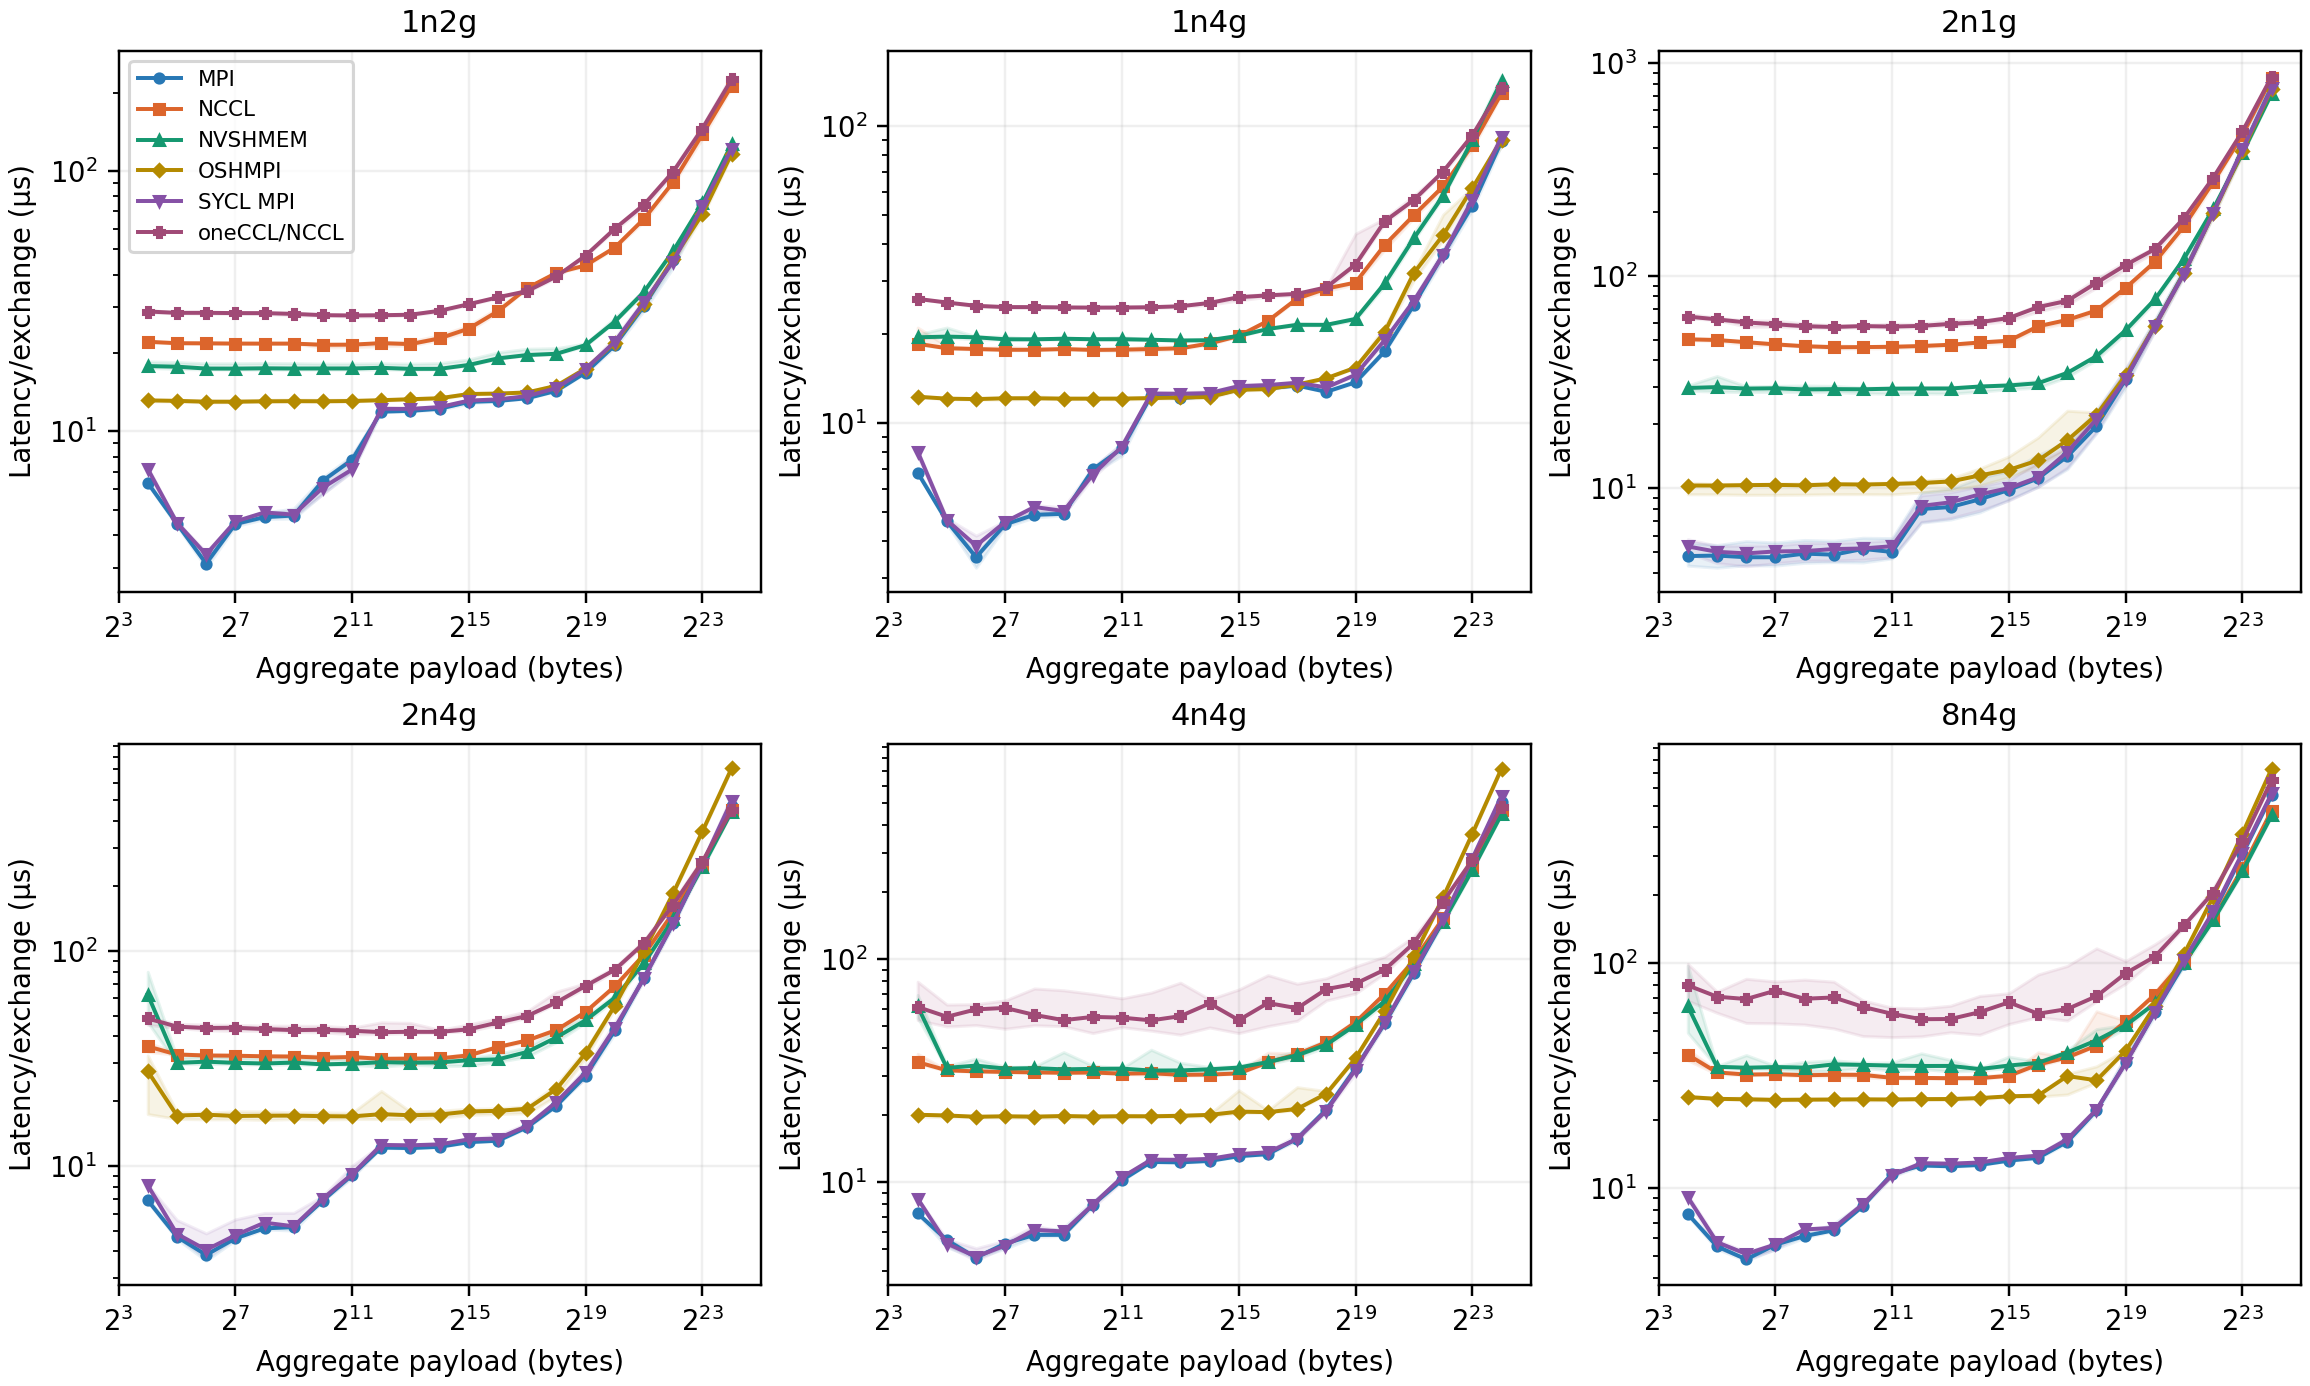
\includegraphics[width=\textwidth]{figures/results/halo-isolated-all-topologies.png}
\caption{Isolated halo latency for all six measured stacks and all six non-single-rank topologies.}
\label{fig:app-halo-isolated}
\end{figure}

\begin{figure}[htbp]
\centering
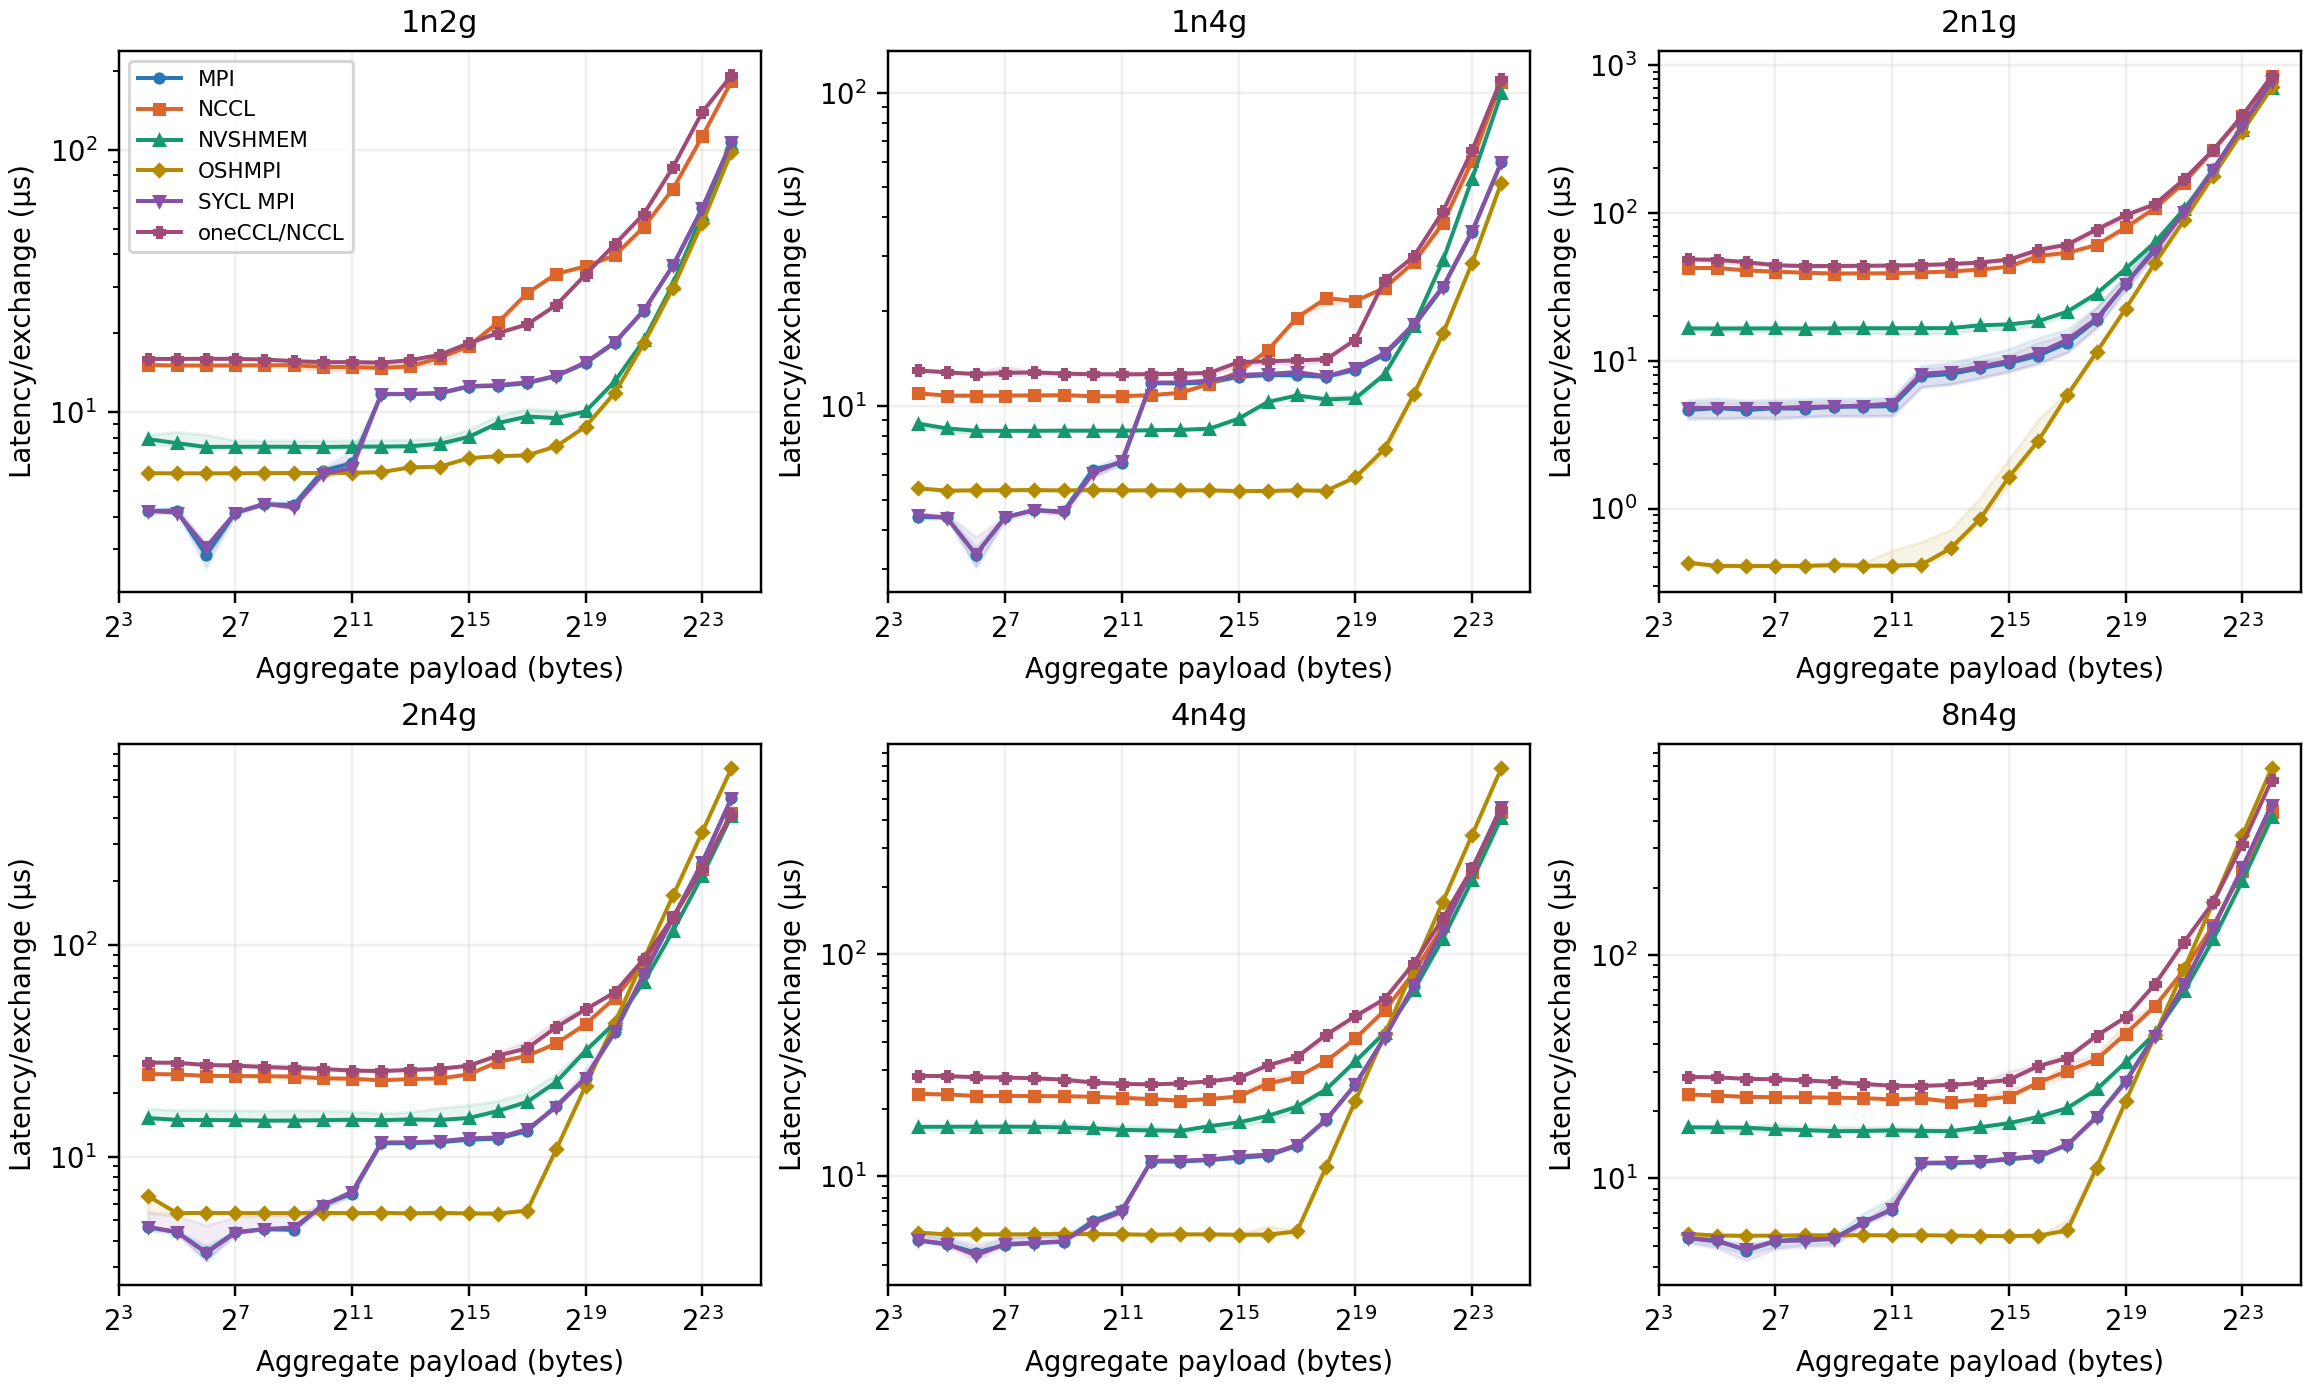
\includegraphics[width=\textwidth]{figures/results/halo-steady-all-topologies.png}
\caption{Steady-state halo latency for all six measured stacks and all six non-single-rank topologies. Values are amortized over batches of 100 exchanges.}
\label{fig:app-halo-steady}
\end{figure}

\section{Collectives}

The single-rank collective panels are implementation controls rather than network baselines. Allreduce uses per-rank input bytes. All-to-all uses bytes per peer, correcting the topology-dependent aggregate-buffer axis in the source analysis artifacts.

\begin{figure}[htbp]
\centering
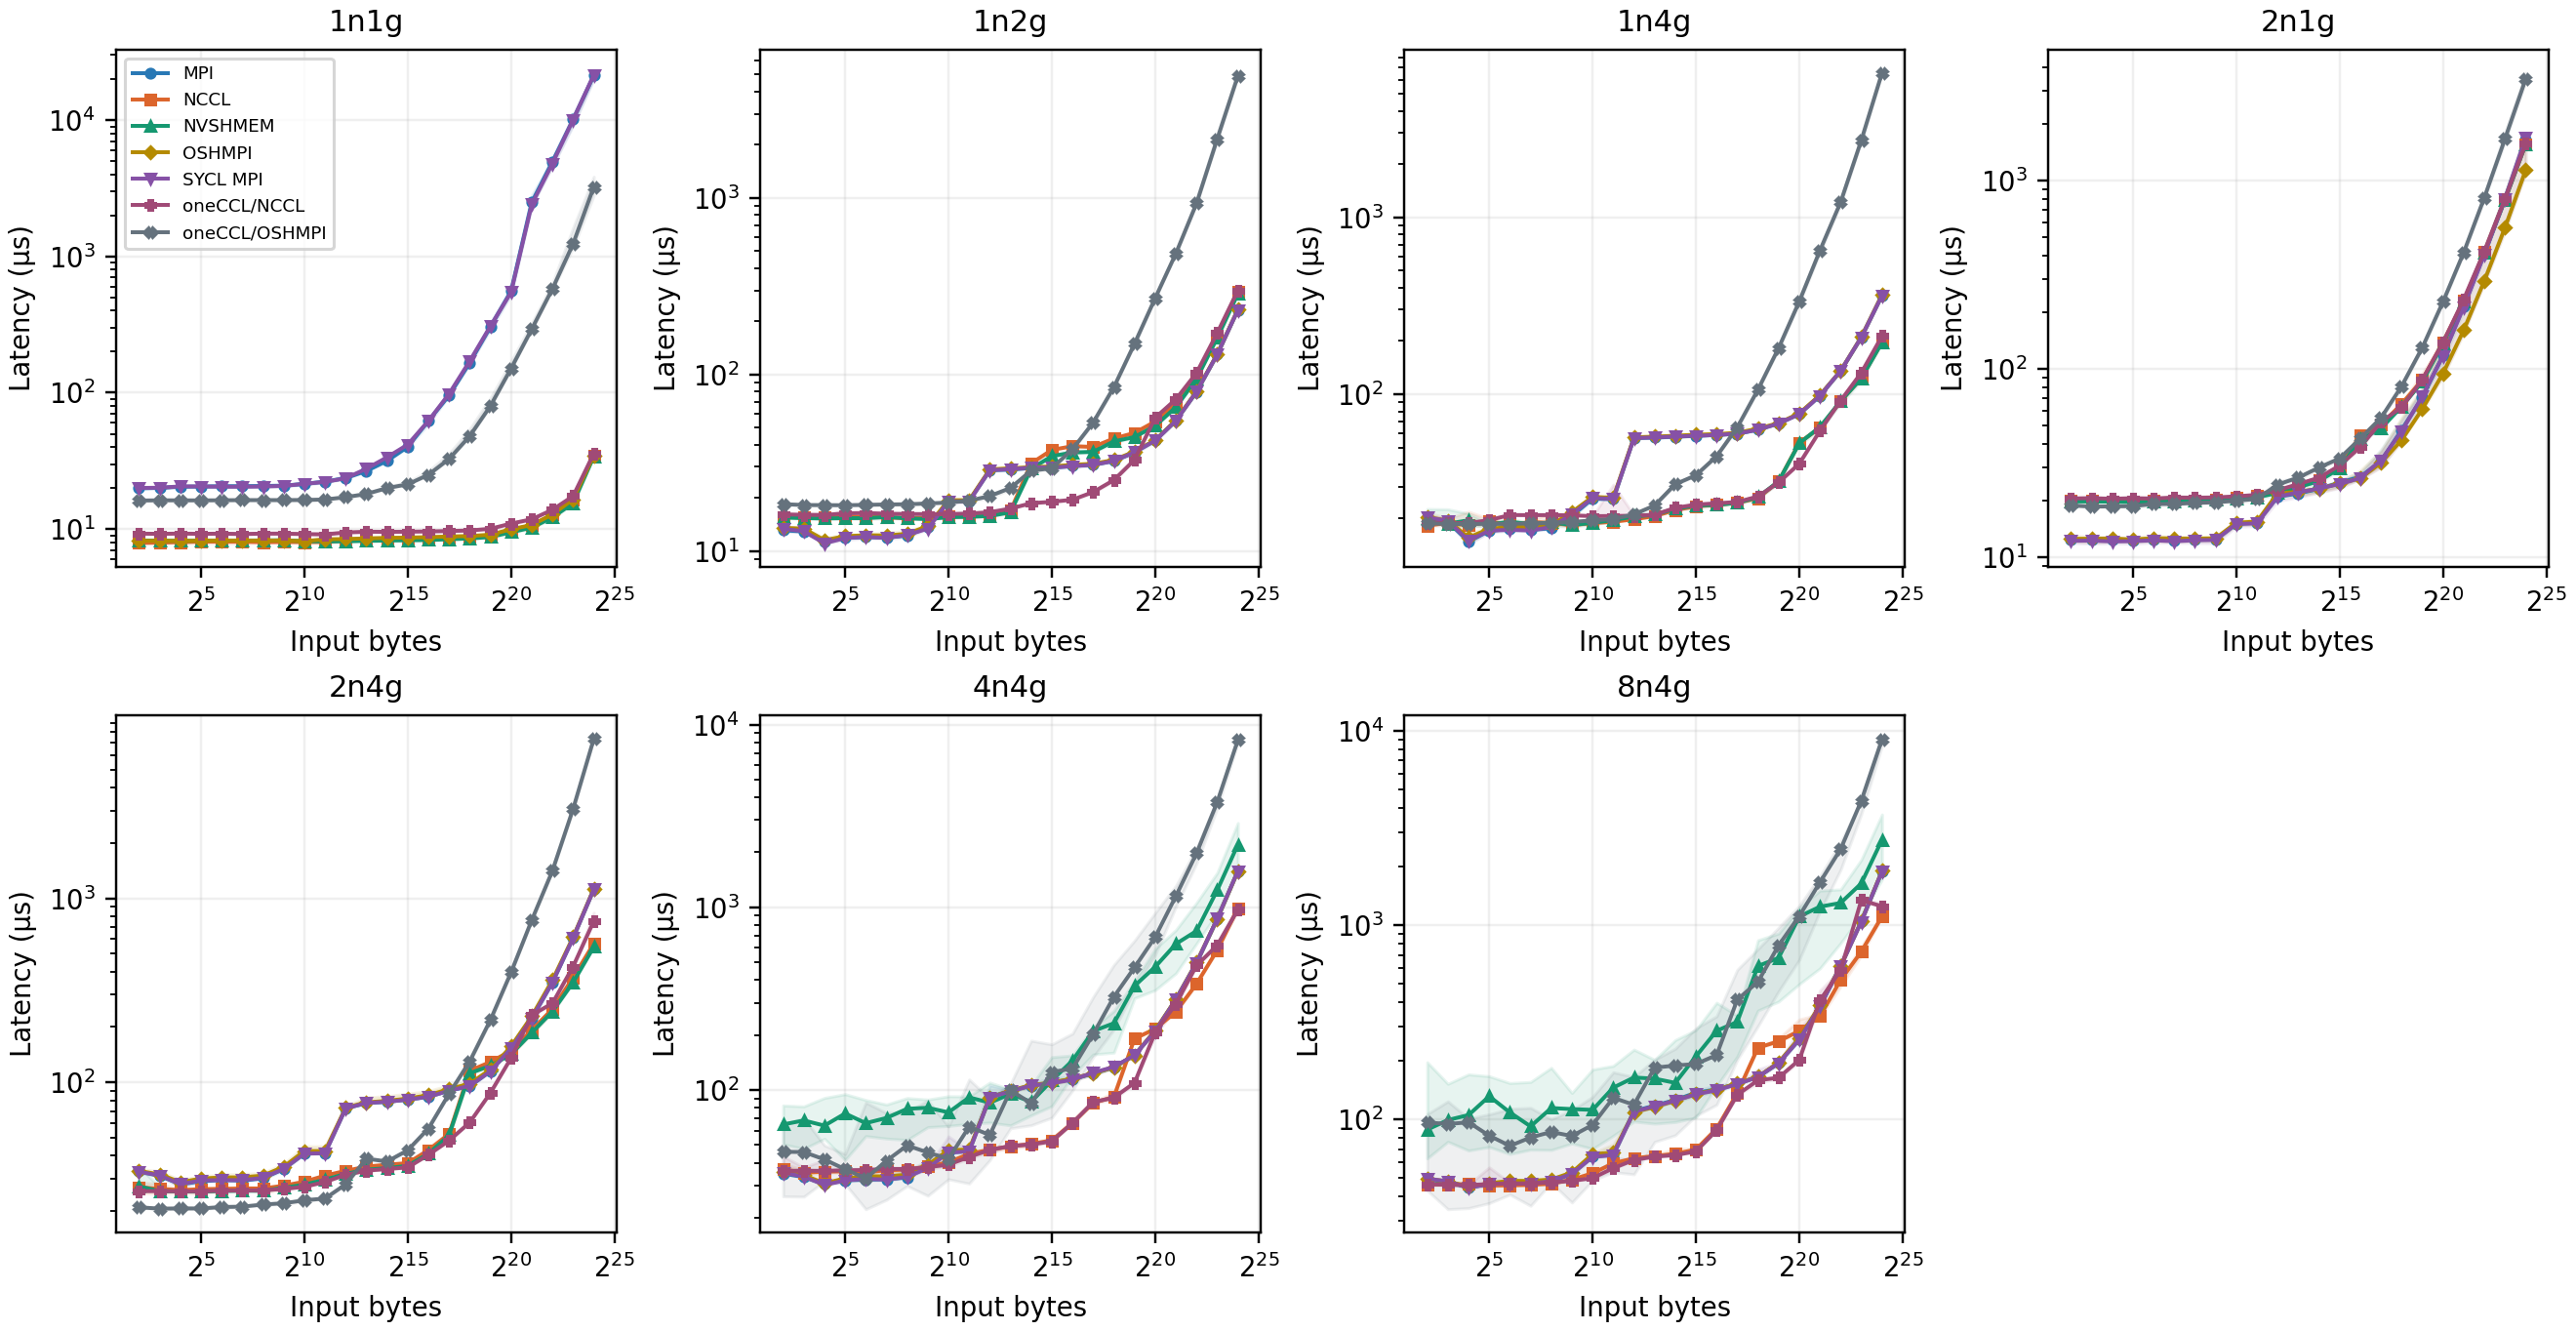
\includegraphics[width=\textwidth]{figures/results/allreduce-all-topologies.png}
\caption{Allreduce latency for all seven measured stacks and all topologies.}
\label{fig:app-allreduce-all}
\end{figure}

\begin{figure}[htbp]
\centering
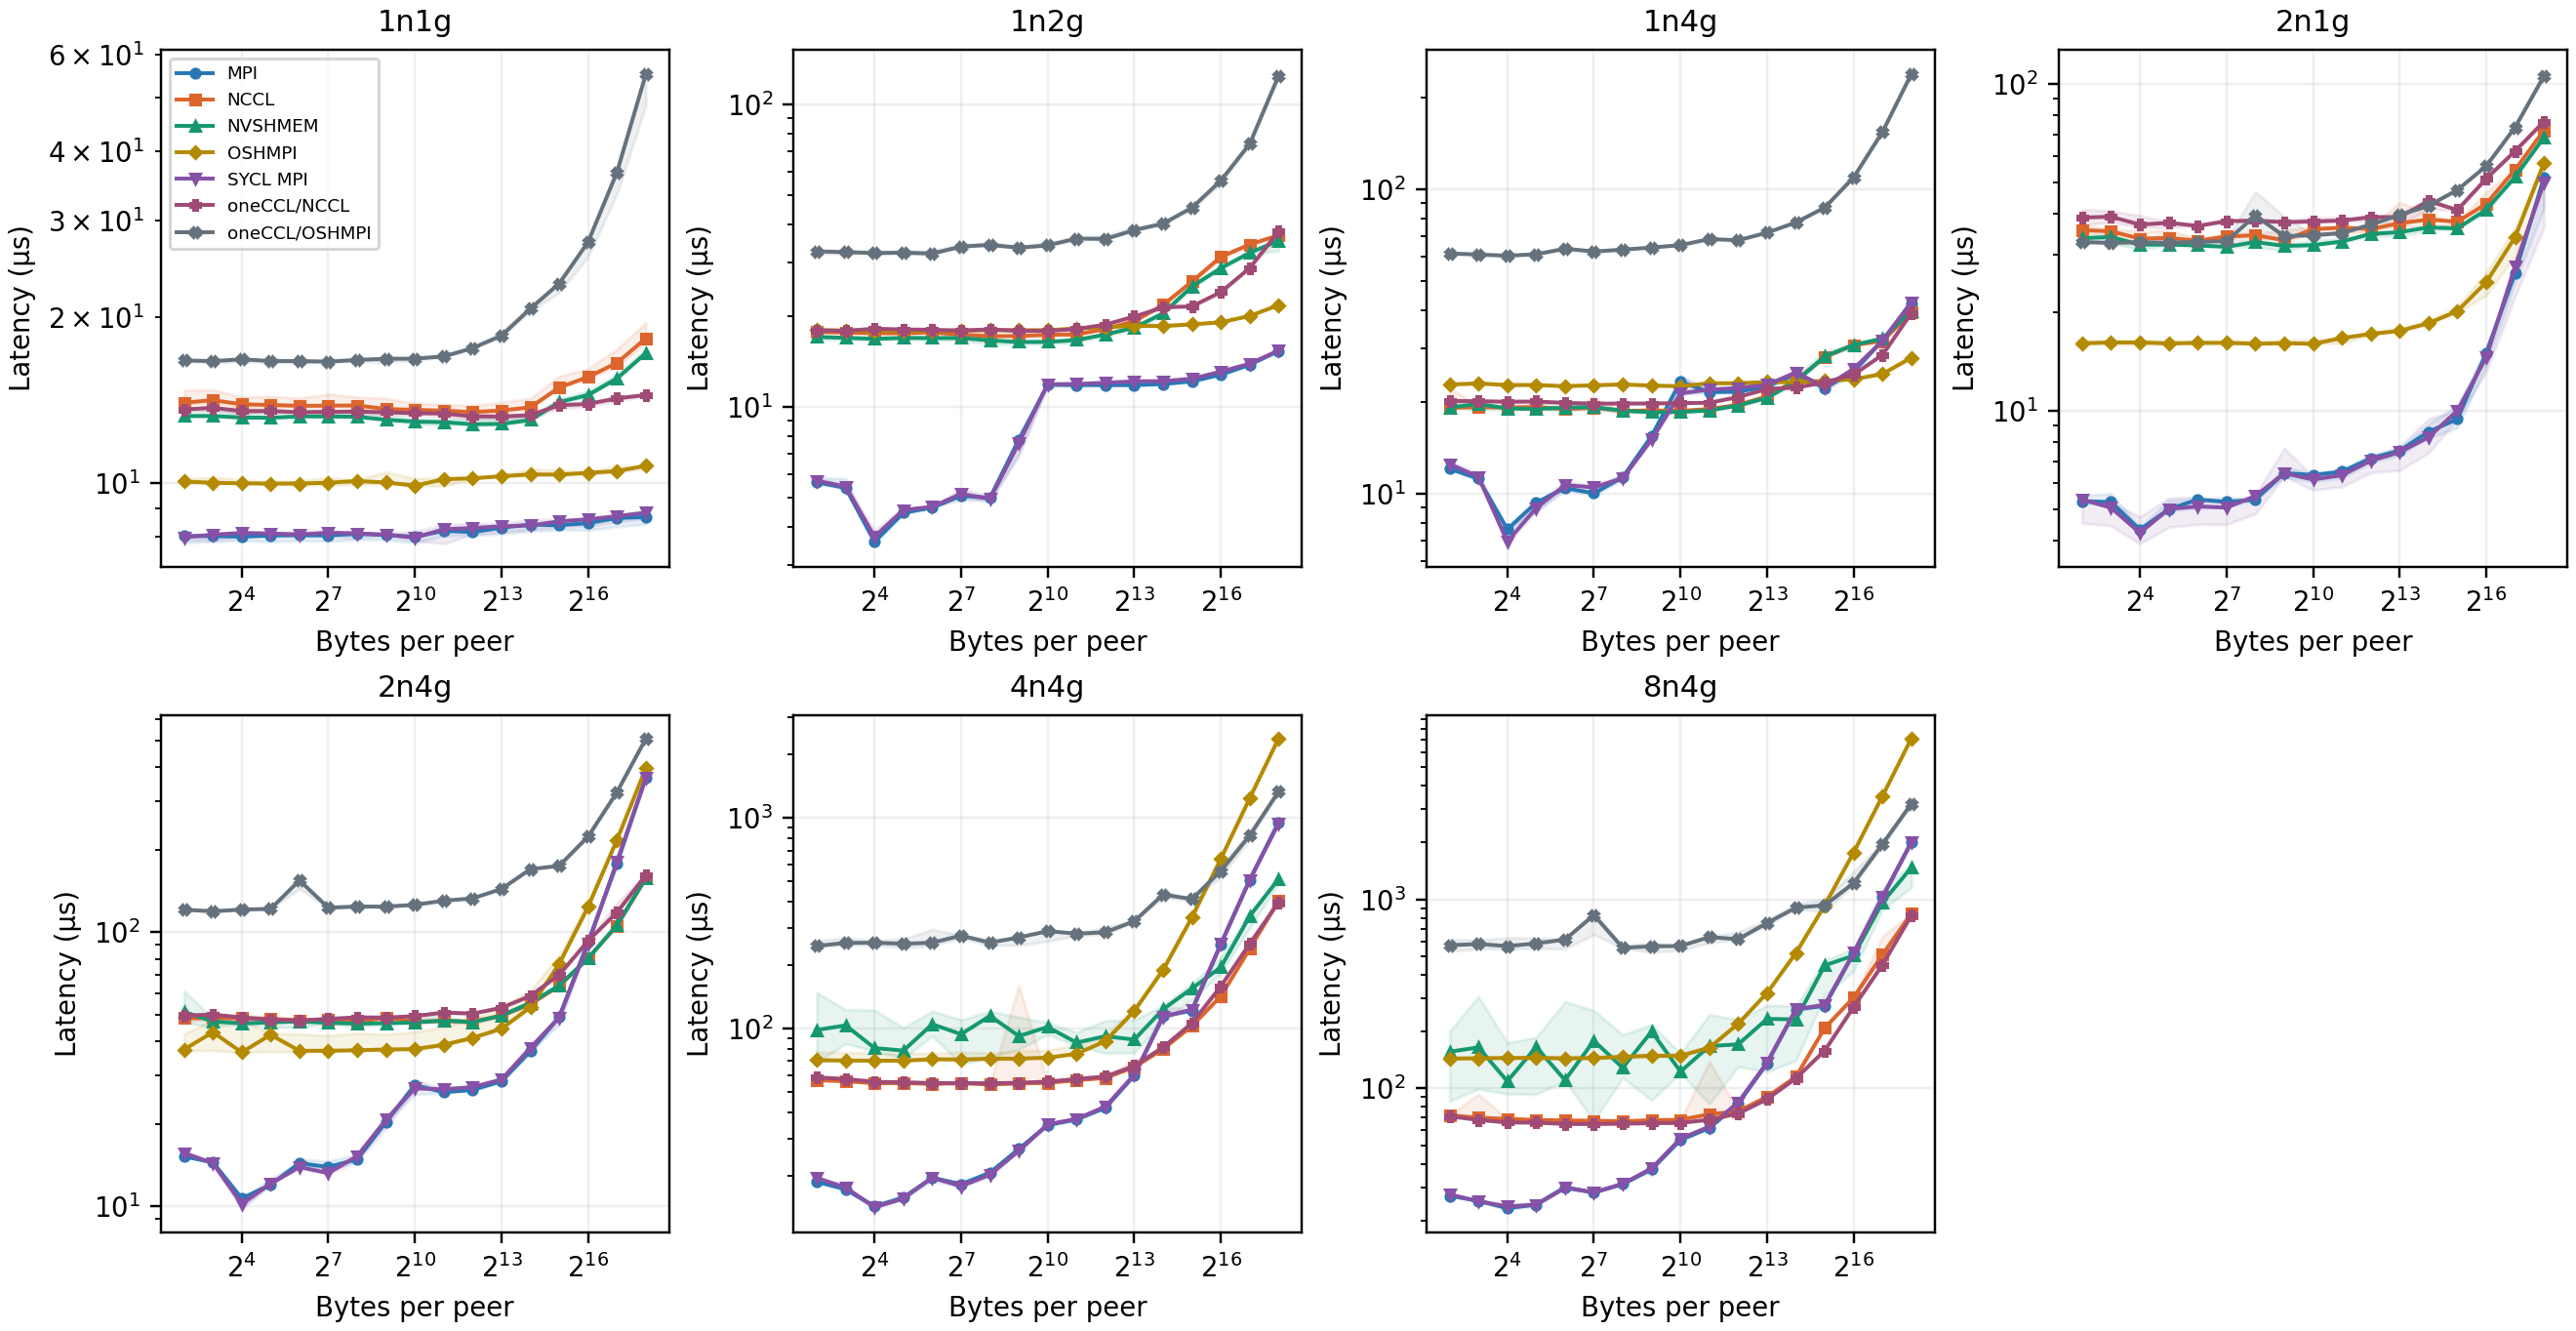
\includegraphics[width=\textwidth]{figures/results/alltoall-all-topologies.png}
\caption{All-to-all latency against bytes per peer for all seven measured stacks and all topologies.}
\label{fig:app-alltoall-all}
\end{figure}

\section{Composite Sequence}

Figure~\ref{fig:app-cg-all} provides every retained \texttt{cg\_step} topology. Ratios use the CUDA MPI median at the same topology and global side as a fixed denominator; the bands do not propagate uncertainty in that denominator. The archived OSHMPI series retains its host-terminal scalar result.

\begin{figure}[htbp]
\centering
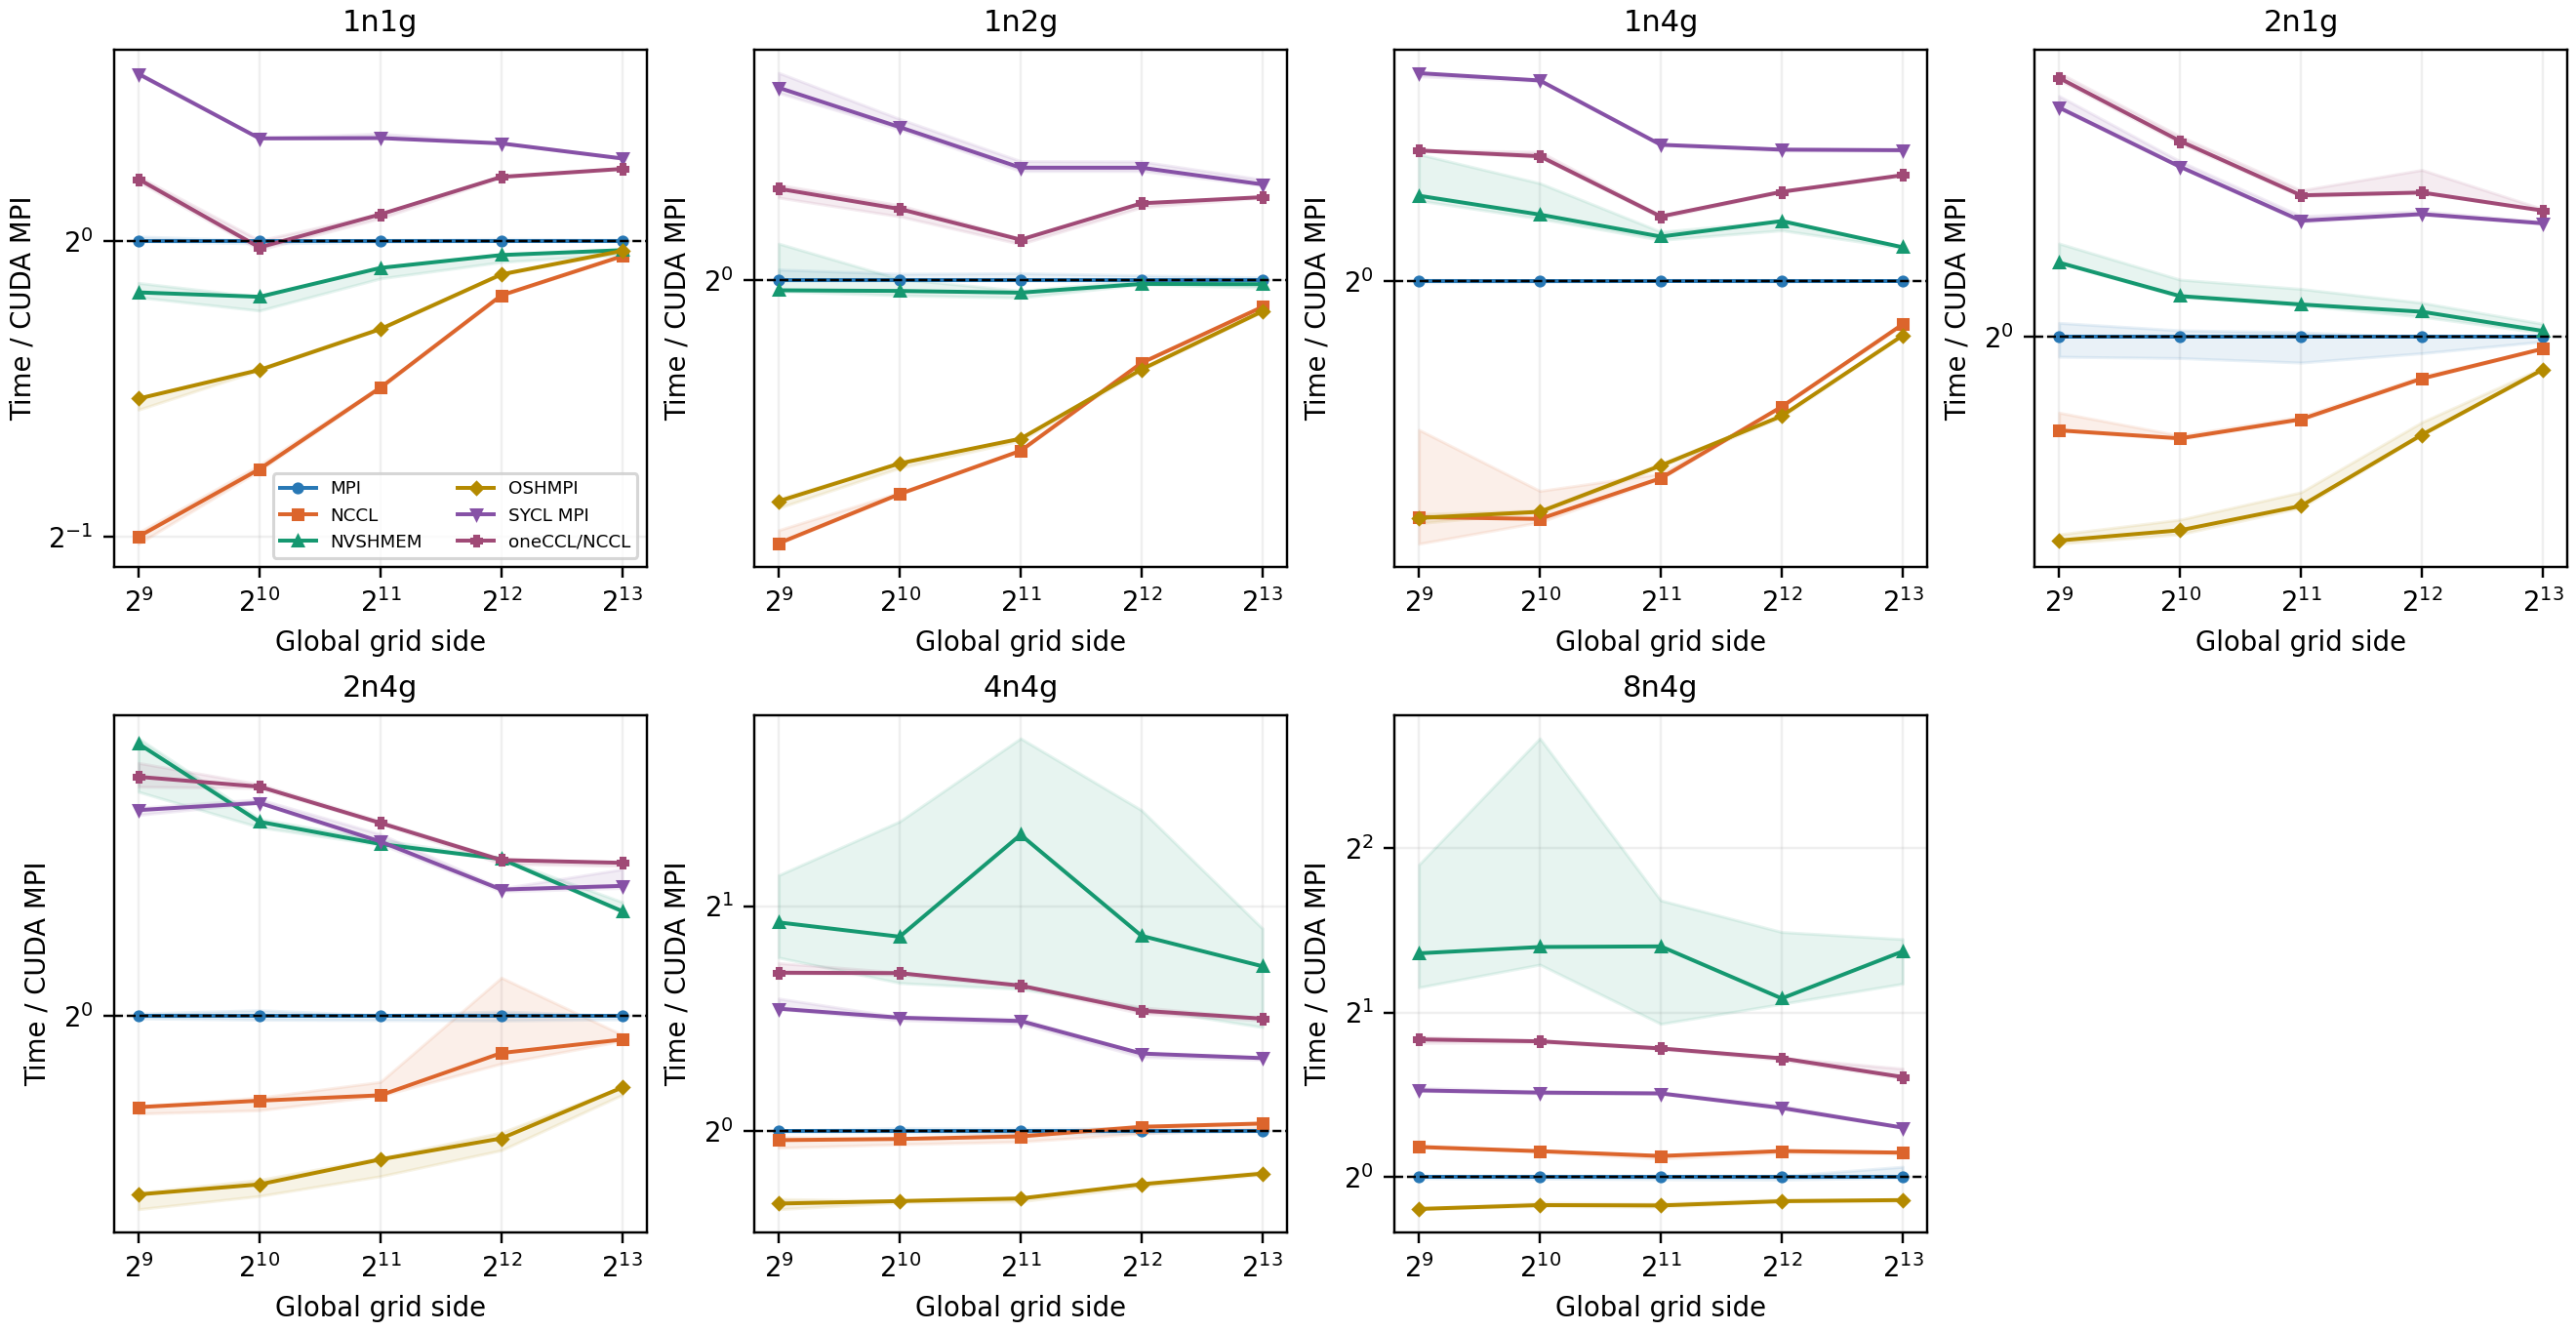
\includegraphics[width=\textwidth]{figures/results/cg-step-all-topologies.png}
\caption{Composite-sequence time relative to CUDA MPI for all six measured stacks and all topologies.}
\label{fig:app-cg-all}
\end{figure}

\chapter{Exploratory NCCL Symmetric-Memory Study}\label{app:nccl-preliminary}

This appendix preserves a later exploratory comparison that is not part of the reconciled main campaign and contributes no evidence to the research-question answers. Its incomplete metadata prevent a device-initiation or application-transfer claim, but the supplied medians identify a candidate for a controlled follow-up.

\section{Protocol and Evidence Boundary}\label{sec:nccl-preliminary-method}

The study compares NCCL~2.18.5 with ordinary allocation, NCCL~2.31.2 with ordinary allocation, and NCCL~2.31.2 with \texttt{ncclMemAlloc} and symmetric window registration on four A100 GPUs. The available summary contains three-run median latencies for 21 allreduce and 19 all-to-all sizes. Comparing versions and comparing the two 2.31.2 configurations answer different questions; the latter still combines allocation and registration.

Symmetric buffers do not establish that user kernels invoked NCCL's device API \cite{nvidia_nccl_registration_2026,nvidia_nccl_device_2026}. Datatype, exact source and launch configuration, completion boundary, warm-up, correctness output, and individual trial timings are unavailable. No uncertainty intervals are reconstructed, and the supplied eight-byte cell is not assumed to be one FP64 sum. The study identifies candidates for follow-up rather than modifying the main campaign's ranking.

\section{Exploratory Results}\label{sec:nccl-preliminary-results}

Table~\ref{tab:m-nccl-preliminary} retains representative gains and regressions from the supplied three-run medians.

\begin{table}[htbp]
\centering
\caption{Preliminary NCCL medians in \,$\mu$s. Plain and symmetric refer to version 2.31.2; the final column divides the 2.18.5 latency by the symmetric latency.}
\label{tab:m-nccl-preliminary}
\footnotesize
\begin{tabular}{llrrrr}
\toprule
Operation & Size & 2.18.5 & Plain & Symmetric & Ratio\\
\midrule
Allreduce & 8\,B & 12.4 & 12.6 & 7.5 & $1.65\times$\\
 & 32\,KiB & 18.4 & 18.5 & 10.6 & $1.74\times$\\
 & 256\,KiB & 19.2 & 19.3 & 22.7 & $0.85\times$\\
 & 1\,MiB & 44.5 & 34.1 & 33.5 & $1.33\times$\\
 & 16\,MiB & 182.0 & 202.1 & 156.4 & $1.16\times$\\
\midrule
All-to-all & 64\,B & 11.1 & 13.8 & 14.0 & $0.79\times$\\
 & 1\,KiB & 11.0 & 12.7 & 12.6 & $0.87\times$\\
 & 8\,MiB & 63.9 & 68.1 & 59.6 & $1.07\times$\\
 & 16\,MiB & 102.2 & 106.1 & 89.2 & $1.15\times$\\
\bottomrule
\end{tabular}
\end{table}

\subsection{Small Allreduce Candidate}

Across the supplied 4\,B--32\,KiB cells, symmetric allocation and registration improve latency by approximately 1.54--1.74 times relative to 2.18.5. At eight bytes the reduction from 12.4 to 7.5\,$\mu$s is approximately 40\% lower latency. Plain 2.31.2 remains at 12.6\,$\mu$s, so the version update alone does not reproduce this small-message gain. The advantage reverses at intermediate sizes, including 256 and 512\,KiB.

\begin{figure}[htbp]
\centering
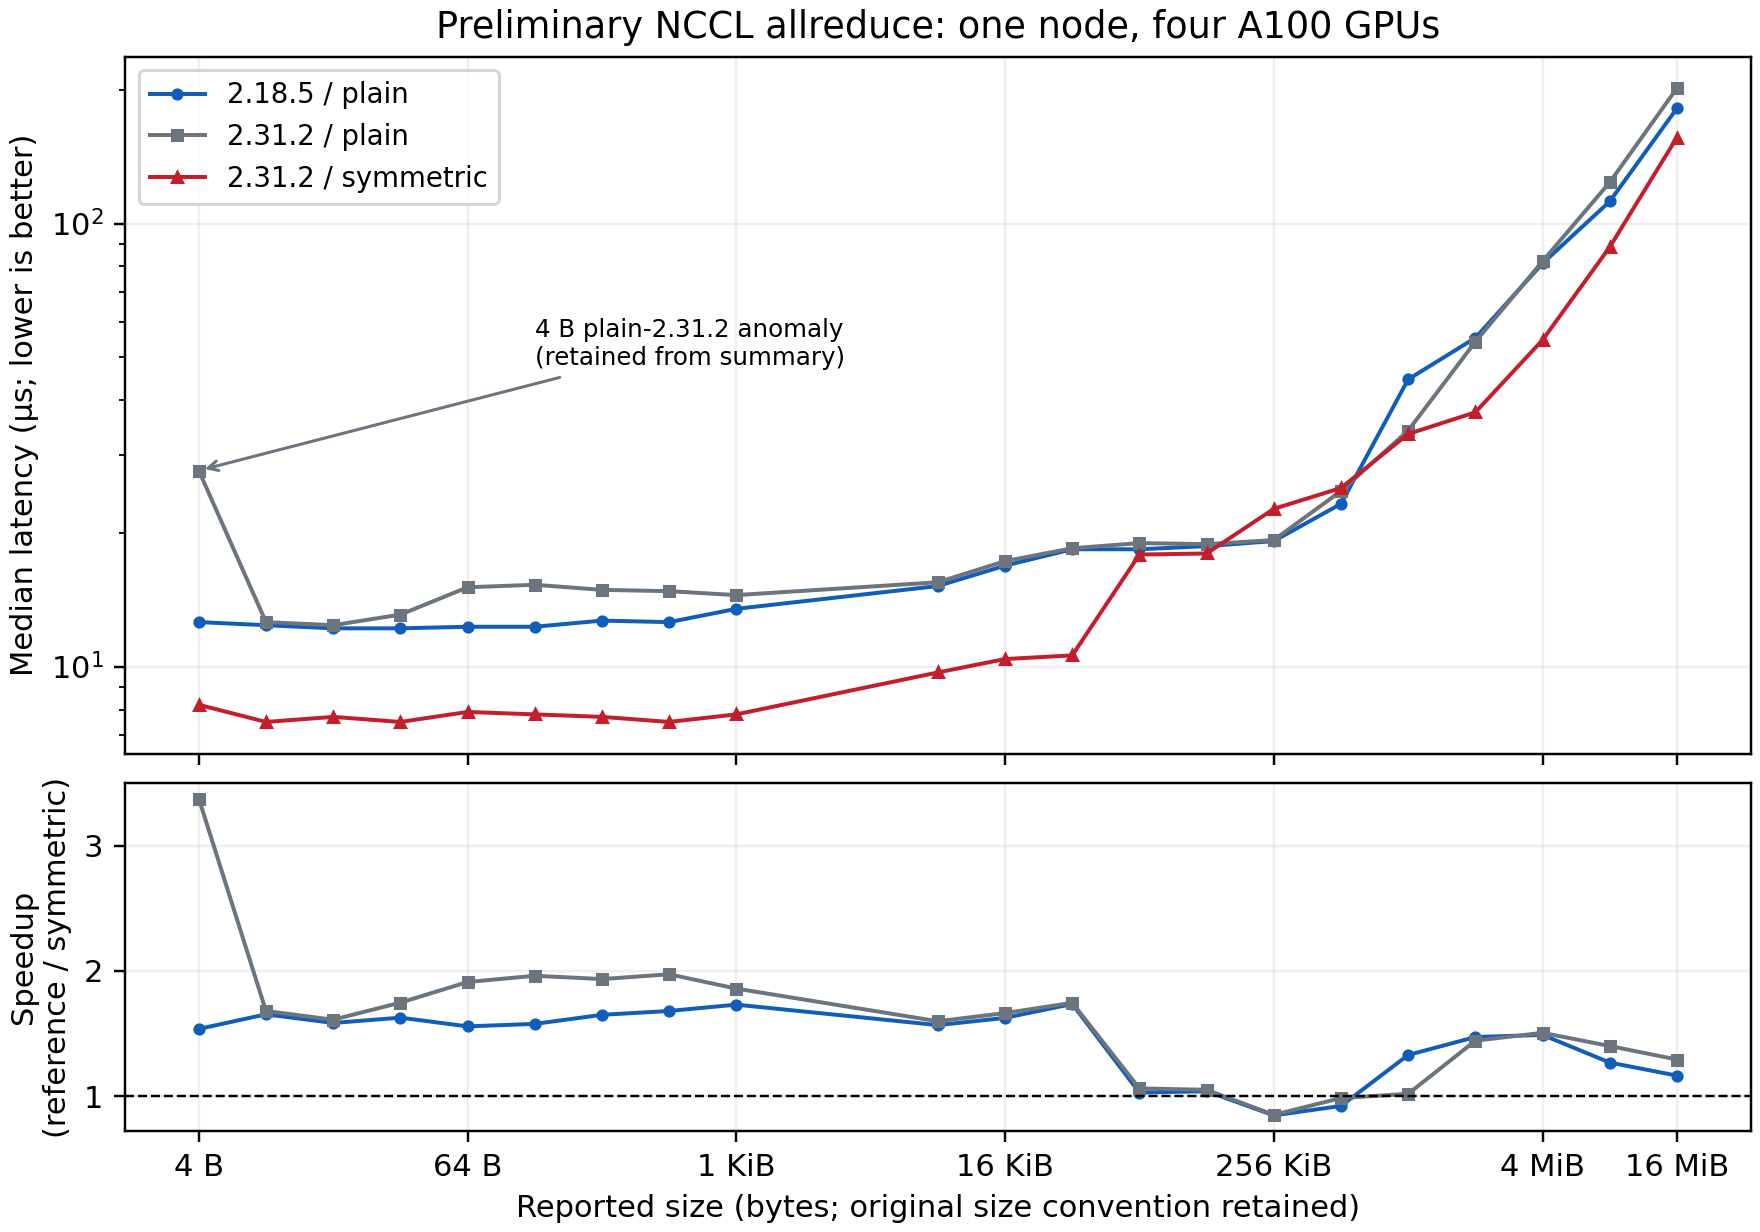
\includegraphics[width=\textwidth]{figures/results/nccl-preliminary-allreduce.png}
\caption{All supplied preliminary allreduce medians. Connecting lines are guides; individual trials and uncertainty intervals are unavailable.}
\label{fig:m-nccl-preliminary-allreduce}
\end{figure}

The eight-byte cell is a candidate for a matched FP64 experiment, not already an estimate of aCG's scalar cost: datatype, invocation mode, and completion boundary remain unresolved.

\subsection{All-to-All Does Not Share the Small-Message Gain}

Small-message all-to-all changes little between the plain and symmetric 2.31.2 configurations, and both are slower than 2.18.5 over the supplied 64\,B--32\,KiB cells. Larger messages show a modest benefit; at 16\,MiB the symmetric configuration is approximately 1.19 times faster than plain 2.31.2.

\begin{figure}[htbp]
\centering
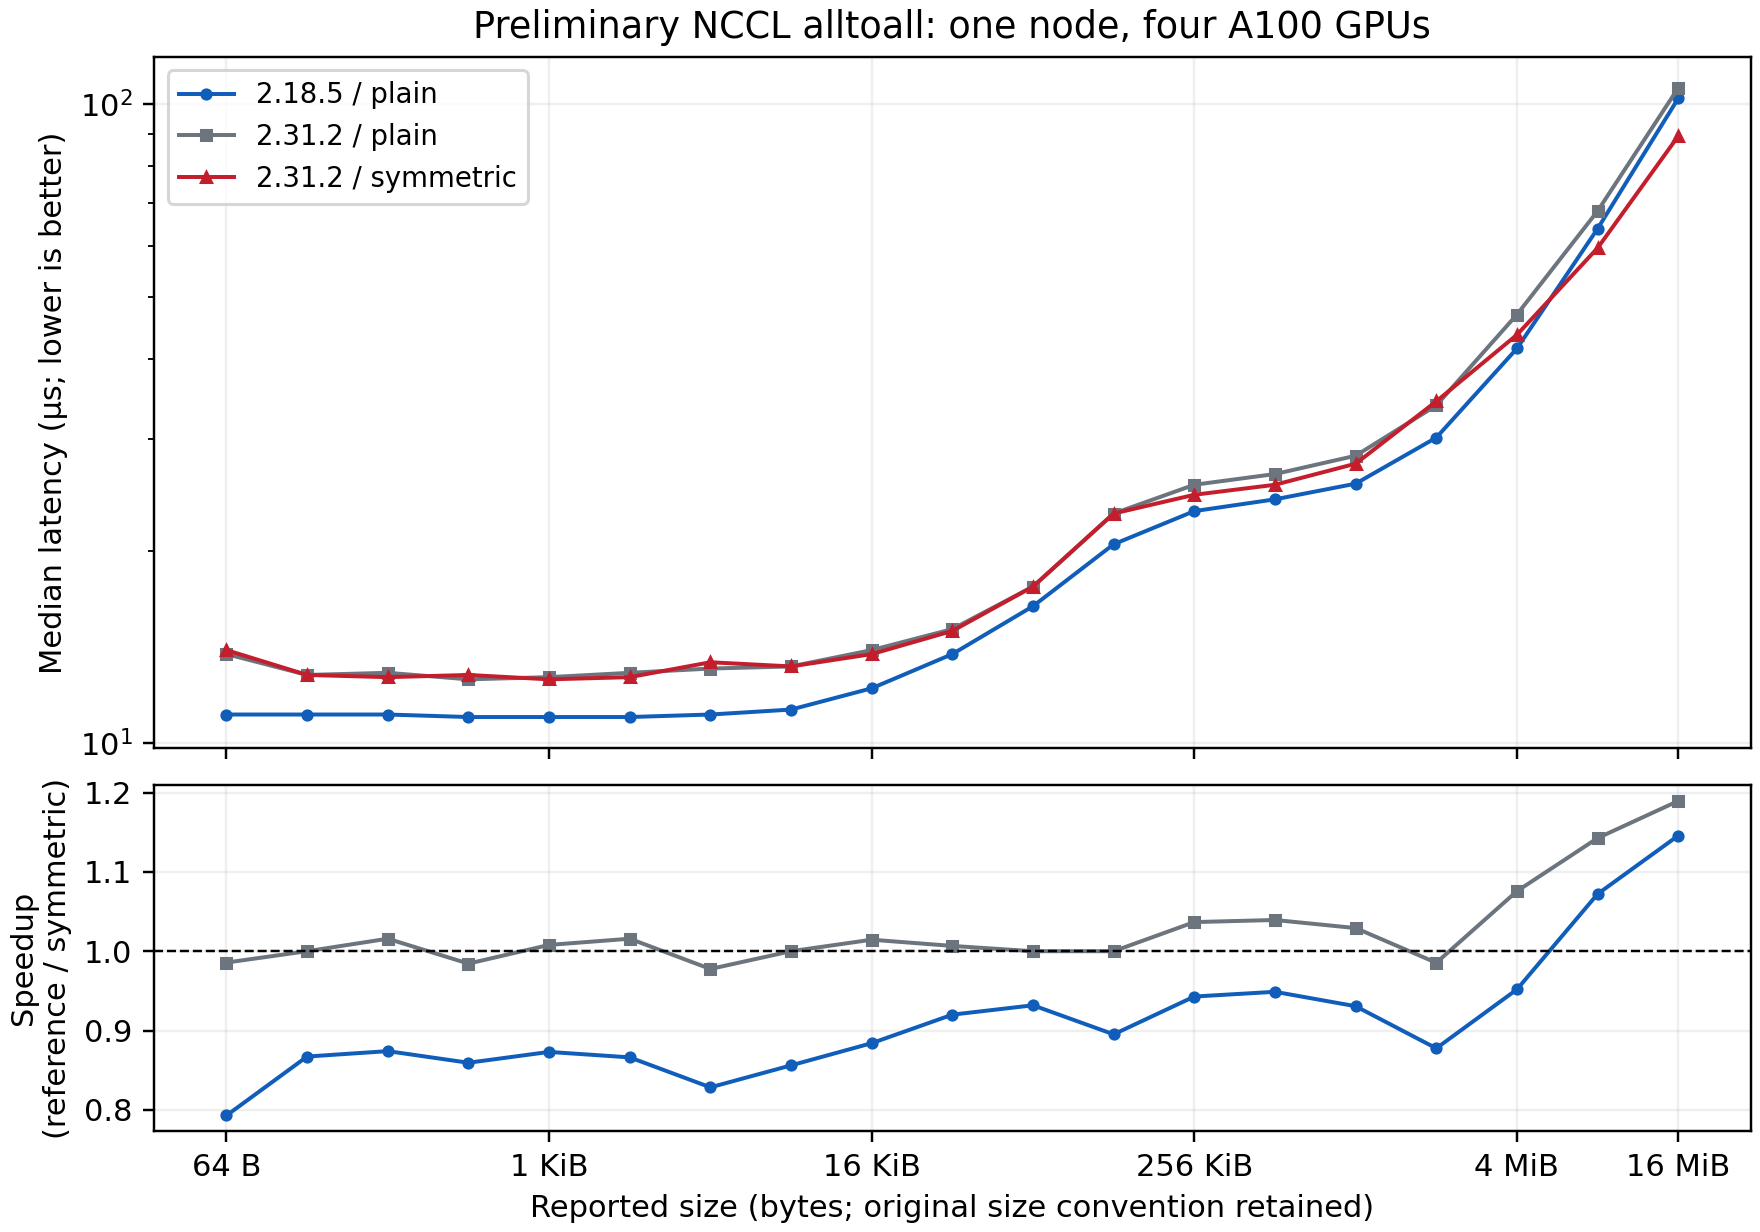
\includegraphics[width=\textwidth]{figures/results/nccl-preliminary-alltoall.png}
\caption{All supplied preliminary all-to-all medians. The size convention is retained from the source summary and is not equated with the main per-peer sweep.}
\label{fig:m-nccl-preliminary-alltoall}
\end{figure}

Source-directory observations alone cannot establish which NCCL kernel produced a timing. Host collectives, grouped point-to-point calls, and user device-API kernels are different paths \cite{nvidia_nccl_collectives_2026,nvidia_nccl_registration_2026}. The reported inter-node proxy regressions and GDAKI stalls lack timing tables and diagnostic logs, so they supply no numerical comparison or established failure cause. The controlled follow-up is a verified one-double intra-node reduction with explicit invocation and completion metadata, followed by an application change only if its benefit persists.


% ---- Back matter ----------------------------------------------------
\printbibliography[heading=bibintoc]

\end{document}
